\pdfoutput=1
\documentclass[11pt]{amsart}
\usepackage{amsmath,amssymb,amsthm,mathtools,mathrsfs}
\usepackage[margin=1.2in]{geometry}
\usepackage{graphicx,booktabs,adjustbox,tikz}
\usetikzlibrary{arrows.meta,positioning,calc}
\usepackage{xcolor,placeins}
\usepackage[colorlinks=true,linkcolor=blue,citecolor=blue,urlcolor=blue]{hyperref}
\hypersetup{pdfauthor={Bernd Johannes Wuebben},pdftitle={Initial conditions and asymptotic phase for Hermitian--Yang--Mills flow}}
\setlength{\emergencystretch}{2em}
\newtheorem{theorem}{Theorem}[section]
\newtheorem{proposition}[theorem]{Proposition}
\newtheorem{lemma}[theorem]{Lemma}
\newtheorem{corollary}[theorem]{Corollary}
\theoremstyle{definition}
\newtheorem{definition}[theorem]{Definition}
\newtheorem{example}[theorem]{Example}
\newtheorem{question}[theorem]{Question}
\theoremstyle{remark}
\newtheorem{remark}[theorem]{Remark}
\newcommand{\CC}{\mathbb C}
\newcommand{\RR}{\mathbb R}
\newcommand{\ZZ}{\mathbb Z}
\newcommand{\PP}{\mathbb P}
\newcommand{\cO}{\mathcal O}
\newcommand{\cI}{\mathcal I}
\newcommand{\db}{\bar\partial}
\newcommand{\tr}{\operatorname{tr}}
\newcommand{\rk}{\operatorname{rk}}
\newcommand{\Hom}{\operatorname{Hom}}
\newcommand{\Coh}{\operatorname{Coh}}
\newcommand{\Vol}{\operatorname{Vol}}
\newcommand{\HYM}{\operatorname{HYM}}
\newcommand{\YM}{\operatorname{YM}}
\newcommand{\Gr}{\operatorname{Gr}}
\newcommand{\id}{\operatorname{id}}
\title[Initial conditions and HYM flow]{Initial conditions and asymptotic phase for Hermitian--Yang--Mills flow}
\author{Bernd Johannes Wuebben}
\subjclass[2020]{53C07 (primary); 14D20, 32G13, 58D27 (secondary)}
\keywords{Hermitian--Yang--Mills flow, invariant manifold, asymptotic phase, stability wall, small eigenvalues}
\date{October 31, 2026\\This version: October 31, 2026}

\newcommand{\End}{\operatorname{End}}
\newcommand{\diag}{\operatorname{diag}}
\newcommand{\ad}{\operatorname{ad}}
\newcommand{\HH}{\mathsf H}
\newcommand{\cK}{\mathcal K}
\newcommand{\cR}{\mathcal R}
\newcommand{\cF}{\mathcal F}
\newcommand{\cD}{\mathscr D}

\newcommand{\cB}{\mathcal B}
\newcommand{\cN}{\mathcal N}
\newcommand{\cH}{\mathcal H}
\newcommand{\cM}{\mathcal M}
\newcommand{\cL}{\mathcal L}
\newcommand{\im}{\operatorname{im}}
\newcommand{\Lie}{\operatorname{Lie}}

\newcommand{\op}{\operatorname{op}}
\newcommand{\supp}{\operatorname{supp}}
\newcommand{\cQ}{\mathcal Q}
\newcommand{\cP}{\mathcal P}
\newcommand{\cV}{\mathcal V}

\begin{document}
\begin{abstract}
We prove that the initial Hermitian metric selects a finite-dimensional
trajectory that tracks Hermitian--Yang--Mills flow with exponentially
decaying relative metric error, uniformly as the positive relaxation
rates separate or tend to zero. The result holds for a nearby stable
family of deformations of a specified sum of four line bundles on the
product of three projective lines, along a fixed polarization path.
We construct an exact invariant graph over the full integrable harmonic
deformation space. Relative to this chosen graph, the asymptotic phase
is continuously differentiable in the initial metric at fixed bundle
and polarization. The local theorem permits bounded diagonal metric
coordinates and sufficiently small transverse displacement. A prescribed
smooth determinant-normalized metric enters this regime after a common
restart time, chosen before the deformation, polarization and
nearby-metric neighborhoods. The proof uses a fixed complementary
spectral gap and metric order, without inverting a small relaxation
rate. For a three-layer family with two independent positive slope
parameters, we also prove all-future comparison with a small,
time-independent relative error.
\end{abstract}

\maketitle


% Source: sections/01_introduction.tex
\section{Introduction}

A finite-dimensional approximation to a geometric flow must record
more than its possible limiting directions. It must identify which
finite trajectory belongs to a prescribed initial metric. This
distinction becomes quantitative near a stability wall: several
finite decay rates can tend to zero at unrelated speeds, while the
directions complementary to the finite model retain a fixed gap.
An initial displacement in those complementary directions can
change the finite trajectory even after the displacement itself
has decayed.

We prove an initial-data-sensitive finite reduction for
Hermitian--Yang--Mills flow near a specified polystable bundle
on $(\PP^1)^3$. The finite coordinates are the complete local
deformation coordinates, including composable extensions and
their analytic obstructions. An exact invariant graph produces
actual metric-flow solutions. A separate phase construction then
selects the graph solution that tracks each nearby actual flow
with exponentially decreasing relative error. The constants do
not involve the inverse of any small finite eigenvalue.

\subsection{Attraction does not determine the finite initial value}
The distinction already occurs in the system
\begin{equation}\label{eq:toy-phase}
 \dot y=-\varepsilon y+av,\qquad
 \dot v=-s v,\qquad 0<\varepsilon<s .
\end{equation}
The invariant line is $v=0$. From $(y_0,v_0)$ its solution is
\[
 v(t)=v_0e^{-st},\qquad
 y(t)=e^{-\varepsilon t}
       \left(y_0+\frac{av_0}{s-\varepsilon}\right)
                -\frac{av_0}{s-\varepsilon}e^{-st}.
\]
The finite solution started at the projected initial value $y_0$
misses a term that decays at the slow rate $\varepsilon$.
The selected initial value is instead
$y_{\rm ph}=y_0+av_0/(s-\varepsilon)$. Its exact finite trajectory
has error $-av_0e^{-st}/(s-\varepsilon)$. The denominator is
controlled by separation from the normal rate, not by
$\varepsilon^{-1}$. Figure~\ref{fig:phase-selection} illustrates
these two choices.

\begin{figure}[tbp]
 \centering
 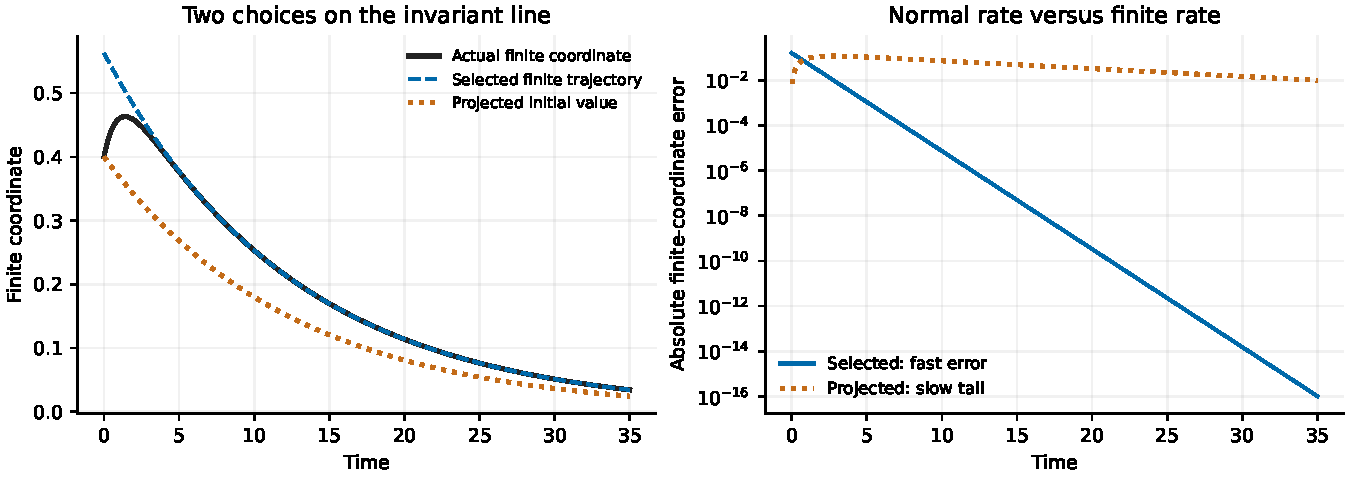
\includegraphics[width=.94\textwidth]{figures/fig01_phase_selection.pdf}
 \caption{Phase selection in \eqref{eq:toy-phase}, with
 $\varepsilon=0.08$, $s=1$, $a=0.3$, $y_0=0.4$, $v_0=0.5$.
 The selected finite solution differs from the actual finite
 coordinate by a fast-decaying term. Starting instead at the
 projected value leaves a slow tail. This exactly solved linear
 system illustrates the distinction; it is not a simulation
 of the geometric flow.}
 \label{fig:phase-selection}
\end{figure}

For a nonlinear finite field with flow $\varphi_t$, the analogous
phase is the limit of $\varphi_{-t}(Y(t))$. Exponential normal
decay makes that limit converge when the finite derivative is
small relative to the fixed normal gap. To prove differentiability
of the phase one must also control the variations of this
infinite-time limit. Finite-time smooth dependence alone does
not provide that conclusion.

\subsection{The geometric result}
The reference bundle is
\[
 E_0=\cO(-2,-2,4)\oplus\cO(1,-2,1)
             \oplus\cO(-2,1,1)\oplus\cO
\]
on $X=(\PP^1)^3$. Its factors have equal slope for the product
polarization. We vary the first two product coefficients along
a signed parameter $l$, with centered slope differences
$l(1,-2/5,0,-3/5)$. The stable-family assertions concern $l>0$.
The determinant metric is fixed. Time is normalized by
\[
 H^{-1}\dot H=-2(i\Lambda_lF_H-\kappa_E(l)I).
\]
Spectra in this paper are those of the complex trace-free
endomorphism Dolbeault Laplacian, with no extra factor two.

The complete harmonic deformation space $V$ has complex dimension
83 and the obstruction space has dimension five. A fixed Hodge
contraction reconstructs $d+a(x)$, with integrability exactly the
convergent equation $\kappa(x)=0$. We retain all higher terms.
The nearby stable HE classes are represented by the corrected
balanced locus $\mathcal B_l^{\rm st}$ of
Section~\ref{sec:geometry}. The complete local quotient and its
coverage are imported, with their hypotheses, from
\cite{WuebbenWall26}; they specify the actual geometric family.

Theorem~\ref{thm:invariant-graph} constructs a chosen finitely
differentiable graph $u=\Psi(l,x)$ in complementary logarithmic
metric coordinates. Its finite equation is exact. On each fixed
stable holomorphic orbit, write $x=e^Y\bar x$, where
$\bar x\in\mathcal B_l^{\rm st}$ and $Y$ is a real trace-free
diagonal. The resulting equation $\dot Y=f_{l,\bar x}(Y)$ has
three real variables. Its reconstruction
$e^{Y\,*}(h_0e^{\Psi(l,e^Y\bar x)})$ solves the metric PDE
exactly, rather than to a finite asymptotic order.

For bounded $Y$ and small complementary displacement,
Theorem~\ref{thm:local-phase} selects a unique trajectory in a
specified fast-tracking class. If $D$ is the initial normal
distance in $h^{17/8}$ and $r$ bounds $|\bar x|$, then
\begin{equation}\label{eq:intro-tracking}
 \begin{gathered}
 e^{-\eta(t)}H_*(t)\le H(t)\le e^{\eta(t)}H_*(t),
       \qquad \eta(t)=CD e^{-ct},\\
 \left|\log\frac{\lambda_j(H(t))}
                       {\nu_j(l,x_*(t))}\right|
       \le Cr^2+CD e^{-ct},\qquad 1\le j\le3,\qquad
 \lambda_4(H(t))\ge\gamma>0 .
 \end{gathered}
\end{equation}
Here $\nu_j$ are the positive eigenvalues of the finite
commutator form on parallel trace-free diagonals. The constants
are independent of their positive ratios. The relative metric
logarithm has the same decaying estimate in $h^{17/8}$, and
the comparison between $H$ and $H_*$ transfers to every positive
Dolbeault eigenvalue. The $Cr^2$ term is a separate static
comparison with the harmonic finite operator.

The phase is $C^1$ in the initial metric at fixed polarization
and balanced base, with uniform derivative bounds in the
declared domains. It is relative to the chosen invariant graph;
neither a canonical graph nor a phase derivative in polarization
is asserted. At equilibrium
Proposition~\ref{prop:equilibrium-rates} identifies the finite
linearized rates exactly as $2\lambda_j(H_{\rm HE})$.
Thus fast attraction to the finite trajectory is compatible
with arbitrarily slow motion along it.

\subsection{Prescribed metrics and independent parameter ranges}
The local initial class can be reached from any prescribed smooth
metric on the fixed underlying bundle. Theorem~\ref{thm:prescribed-phase}
has the following order of choices. Fix that metric, a graph and
a requested entry accuracy. First choose a finite reference
restart. Then choose sufficiently small polarization and
deformation neighborhoods and a strong neighborhood of the
prescribed metric. Every stable balanced point and every initial
metric in those neighborhoods enter the phase theorem at that
same restart. The phase remains $C^1$ in the initial metric.
Only the finite ODE is continued backward if its selected initial
value is to be expressed at the original time zero.

The reference entry proof needs both metric convergence in a
fixed presentation and strong finite-time dependence. Connection
convergence modulo gauge does not directly imply the former.
For the split reference bundle, metric order bounds the convergence
gauges; elliptic compactness then identifies a limiting positive
diagonal metric. The unsliced logarithmic equation supplies
finite-time dependence in the full $h^{19/8}$ domain. These
arguments are given in Section~\ref{sec:entry}.

A second application retains two independent positive slope
parameters $k,l$ on a three-layer diamond. Its four adjacent
arrows compose nontrivially, and a quadratic central Hodge
primitive is necessary for integrability. The total arrow
energy confines its finite dynamics by a height identity.
Theorem~\ref{thm:diamond-comparison} gives all-future relative
metric and three-mode comparison from an open initial class,
without a lower bound on $k/l$. Its explicit example has one
eigenvalue asymptotic to $k$ and two of order $l$ as $k/l\to0$.

For this fixed diamond bundle,
Theorem~\ref{thm:diamond-prescribed} allows arbitrary smooth
prescribed initial metrics, after a common restart on a full
positive parameter triangle. Its error is a controllably small
constant. The proof recovers the three filtration layers from
normalized holomorphic maps, removes exact adjacent and central
entries, and proves exact diagonal-orbit matching. It does not
produce the differentiable phase of the complete-family theorem.
Section~\ref{sec:compatibility} identifies the overlap of the
two descriptions along $k=3l/5$, including their actual metric
and finite spectral comparisons.

\subsection{Relation to earlier work and proof structure}
Finite-dimensional reductions and initial-data-dependent asymptotic
trajectories have an established role in geometric flow.
Haiden, Katzarkov, Kontsevich and Pandit study finite gradient
flows and iterated logarithmic asymptotics and prove the
metric-order principle used here \cite{HKKP18}.
Lam gives a finite reduction and bounded-distance comparison
for HYM flow of semistable bundles with locally free graded
object, together with an equivariant Kuranishi description
\cite[Proposition 8.6 and Theorem 8.7]{Lam26}.
These results are direct predecessors. Our assertion is a
decaying near-one relative metric comparison, with differentiable
phase and uniformity through the stated collapsing finite scales.

The invariant-graph input is Simonett's theorem for parabolic
equations \cite[Theorem 2.1]{Simonett94}. Its attraction estimate
concerns distance to the graph over the current finite coordinate;
we separately select and differentiate the tracking trajectory.
The proof is an application of established invariant-manifold
and asymptotic-phase ideas, with the quantitative estimates
needed for the present geometric degeneration printed in full.
Shao--Simonett supplies the normally elliptic realization and
continuous maximal regularity \cite{ShaoSimonett14}, while
Simonett's local semiflow theorem includes the strong initial
topology needed for finite-time entry \cite{Simonett95}.

For two-step extensions, \cite[Sections 6 and 8]{WuebbenFlow26}
already constructs exact invariant-graph flows and proves
prescribed-metric matching with all-future comparison after
restart. The additions here are the complete composable
deformation family, the phase with decaying relative error and
its differentiability, and the three-layer geometric matching
needed for the independent two-parameter application.
Stationary metric and spectral estimates are imported only
in their stated scope from \cite{WuebbenThreeStep26,WuebbenWall26}.
They do not supply parabolic invariance or phase selection.

Sections~\ref{sec:geometry}--\ref{sec:reduction} establish the
geometric interface and exact finite graph.
Section~\ref{sec:abstract-phase} proves the reusable phase
estimate, and Sections~\ref{sec:geometric-phase}--\ref{sec:entry}
give its geometric realization and prescribed entry.
Section~\ref{sec:spectra} separates nonstationary spectral
comparison from equilibrium rates.
Sections~\ref{sec:diamond}--\ref{sec:compatibility} retain the
two-parameter application and compare the overlapping descriptions.

% Source: sections/02_geometry.tex
\section{The complete deformation family}\label{sec:geometry}

The finite coordinates used below describe holomorphic bundles, whereas
the finite evolution stays on one holomorphic orbit. We first specify
that distinction and the geometric neighborhood in which the estimates
will be uniform.

\subsection{The split bundle and the polarization}
Let $X=(\PP^1)^3$, and let $\omega_i$ be the product
Fubini--Study forms, normalized by $\int_{\PP^1}\omega_i=1$.
Set
\begin{equation}\label{eq:factors}
 F_1=\cO(-2,-2,4),\quad F_2=\cO(1,-2,1),\quad
 F_3=\cO(-2,1,1),\quad F_4=\cO,\qquad E_0=\bigoplus_{i=1}^4F_i.
\end{equation}
Write $h_0$ for the orthogonal product metric, $A_0$ for its Chern
connection, and $d$ for the split Dolbeault operator and its induced
operators on endomorphism-valued forms. A block $ij$ maps $F_j$ to $F_i$.
The determinant line is $\cO(-3,-3,6)$. Throughout the paper its
metric is fixed to be $\det h_0$.

For the complete family, the polarization follows the path
\begin{equation}\label{eq:polarization}
 \omega_l=h_1(l)\omega_1+h_2(l)\omega_2+\omega_3,\qquad
 h_1(l)=\left(1+\frac{7l}{30\pi}\right)^{-1},\quad
 h_2(l)=\left(1+\frac{l}{6\pi}\right)^{-1}.
\end{equation}
It is K\"ahler on an open interval about $l=0$. The parabolic
construction uses this signed interval; the stable-family conclusions
use $l>0$. All squared $L^2$ norms are divided by
$\Vol_l=h_1h_2$. The resulting spatial measure is independent of $l$.
If $\kappa_i(l)=i\Lambda_lF_{F_i,h_i}$ and
$\kappa_E=\frac14\sum_i\kappa_i$, then
\begin{equation}\label{eq:slopes}
 b(l)=(\kappa_E-\kappa_i)_{i=1}^4
       =l(1,-2/5,0,-3/5).
\end{equation}
The product determinant metric has constant contracted curvature
$4\kappa_E(l)$ even though its line bundle is nontrivial.

Let
\[
 \mathfrak t=\{\xi\in\CC^4:\textstyle\sum_i\xi_i=0\},\qquad
 \mathfrak t_{\RR}=\mathfrak t\cap\RR^4,\qquad
 |\xi|^2=\sum_i|\xi_i|^2.
\]
These are the parallel trace-free diagonal endomorphisms and their
Hermitian part. There are no other split holomorphic endomorphisms:
every nonzero difference of the degree triples in \eqref{eq:factors}
has sum zero and a negative entry, so its product line bundle has
no section. Let $\mathcal V$ be the real bundle of $h_0$-Hermitian
trace-free endomorphisms. On its sections let $P_0$ be normalized
$L^2$ projection onto $\mathfrak t_{\RR}$, and set $Q_0=1-P_0$.
The projections are fixed as $l$ varies.

\subsection{Reconstruction and the actual HE neighborhood}
Use the reference geometry at $l=0$ to define harmonic projections
$P_j$, harmonic inclusion $\iota$, and the Hodge homotopy $K=d^*G$.
Put $V=H^1(X,\End_0E_0)$. Its nine nonzero blocks are
\begin{equation}\label{eq:harmonic-blocks}
\begin{array}{c|ccc|ccc|ccc}
 ij&12&32&34&13&23&24&21&31&41\\ \hline
 \dim_{\CC}V_{ij}&8&8&4&8&8&4&8&8&27\\
 \text{differential factor}&1&1&1&2&2&2&3&3&3
\end{array}
\end{equation}
Thus $\dim_{\CC}V=83$, while $H^2(X,\End_0E_0)$ has dimension five
and is supported in block $14$. These dimensions follow from
K\"unneth and line-bundle cohomology, as computed in
\cite[Sections 3 and 5]{WuebbenWall26}. The representatives in
\eqref{eq:harmonic-blocks} remain harmonic for every $\omega_l$.
Their normalized squared norm is
\begin{equation}\label{eq:harmonic-norm}
 \begin{split}
 q_l(x)=\|\iota x\|_l^2={}&
 h_1^{-1}(\|x_{12}\|_0^2+\|x_{32}\|_0^2+\|x_{34}\|_0^2)\\
 &+h_2^{-1}(\|x_{13}\|_0^2+\|x_{23}\|_0^2+\|x_{24}\|_0^2)\\
 &+\|x_{21}\|_0^2+\|x_{31}\|_0^2+\|x_{41}\|_0^2.
 \end{split}
\end{equation}
Write $|x|=\|\iota x\|_0$.

We recall precisely the stationary geometric input. A constant
invertible diagonal $g$ acts by $(gx)_{ij}=g_i g_j^{-1}x_{ij}$.
Its infinitesimal action is
\begin{equation}\label{eq:orbit-map}
 C_x\xi=((\xi_i-\xi_j)x_{ij})_{ij}.
\end{equation}

\begin{proposition}[Complete local model, \cite{WuebbenWall26}]
\label{prop:geometric-input}
On a fixed coefficient ball there is a convergent holomorphic
reconstruction
\begin{equation}\label{eq:reconstruction}
 a(x)=\iota x-K(a(x)^2),\qquad
 \kappa(x)=P_2(a(x)^2),\qquad d_x=d+a(x).
\end{equation}
The operator $d_x$ is integrable exactly when $\kappa(x)=0$.
The five-component equation retains all higher terms. The map $a$
is equivariant under constant diagonals wherever both arguments lie
in its domain, and every holomorphic map between sufficiently small
integrable reconstructed objects is such a constant intertwiner.

For the centered curvature
\begin{equation}\label{eq:centered-curvature}
 \mathcal M(l,x,u)=
 e^{u/2}i\Lambda_lF_{d_x,h_0e^u}e^{-u/2}-\kappa_E(l)I
\end{equation}
there is a unique small complementary solution $w(l,x)$ of
$Q_0\mathcal M(l,x,w)=0$, $P_0w=0$. It is smooth and
$O(|x|^2)$ in every fixed finite spatial norm. Define
\begin{equation}\label{eq:balanced-domain}
 m_l(x)=P_0\mathcal M(l,x,w(l,x)),\qquad
 \mathcal B_l(r)=\{x:|x|<r,\ \kappa(x)=0,\ m_l(x)=0\}.
\end{equation}
For $0\le l\le l_0$, its compact diagonal quotient identifies with an
open neighborhood of actual fixed-determinant HE classes. For fixed
$s\ge6$ there are uniform $c_0,C_0>0$ such that this image contains
every such class having a unitary representative
$\|A-A_0\|_{H^s}<c_0r$, and every point of the image has a
representative with $\|A-A_0\|_{H^s}<C_0r$.
\end{proposition}

The proposition is \cite[Sections 6 and 9]{WuebbenWall26}, including
its geometric coverage and compact-orbit uniqueness. The reconstruction
uses a fixed reference contraction and is independent of $l$.
The complementary equation extends to signed $l$ by the same
parameter implicit-function theorem. We do not infer a parabolic
invariance assertion from that elliptic equation.

Here are two estimates from the reconstruction that will be used
explicitly. With $J_x=D_xa$,
\begin{equation}\label{eq:harmonic-orthogonality}
 J_xv=\iota v+B_xv,\qquad
 \langle\iota v,B_xv'\rangle_l=0,\qquad
 \|B_xv\|_{H^s}\le C_s|x||v|.
\end{equation}
Indeed differentiating \eqref{eq:reconstruction} puts the correction
in the reference coexact space. Pairing with any harmonic block for
$\omega_l$ multiplies its reference pairing by the corresponding
scalar in \eqref{eq:harmonic-norm}; it remains zero. Integration
along a radial segment gives the same orthogonality for
$a(x)-\iota x$. Equivariance also gives, exactly,
\begin{equation}\label{eq:equivariant-derivative}
 d_x^{\End}\xi=-J_xC_x\xi .
\end{equation}

The support graph has vertices $1,2,3,4$ and an undirected edge
between $i,j$ whenever $x_{ij}$ or $x_{ji}$ is nonzero.
Let $\mathcal B_l^{\rm st}(r)$ be the connected-support part of
\eqref{eq:balanced-domain}. Its bundles are stable: they are HE,
and the constant-intertwiner assertion makes their trace-free
holomorphic kernel zero. Conversely this is the stable part of
the declared local HE quotient. No smoothness or rank condition
on $\kappa^{-1}(0)$ is imposed.

\subsection{Metric and spectral conventions}
Each flow fixes $l$, its holomorphic bundle, and the determinant.
Its time normalization is
\begin{equation}\label{eq:hym-flow}
 H^{-1}\partial_tH=-2(i\Lambda_lF_H-\kappa_E(l)I).
\end{equation}
All spectral statements concern
$\Delta_{\bar\partial,H}=\bar\partial_{\End_0}^*
\bar\partial_{\End_0}$ on complex trace-free endomorphism zero-forms,
without a factor two, with complex multiplicities and zeros counted.
The finite Hermitian operator on $\mathfrak t$ is
\begin{equation}\label{eq:finite-operator}
 \langle\xi,L_{{\rm fin},l}(x)\xi\rangle
   =\|C_x\xi\|_l^2
   =\sum_{ij}\|x_{ij}\|_l^2|\xi_i-\xi_j|^2.
\end{equation}
Its three ordered eigenvalues are $\nu_1(l,x),\nu_2(l,x),\nu_3(l,x)$.
They are positive precisely when the support is connected.

For positive metrics on the same bundle define
\begin{equation}\label{eq:order-distance}
 d_\infty(H,K)=\sup_{p\in X}\max_j
       |\log\lambda_j(H_p^{-1}K_p)|.
\end{equation}
Equivalently $d_\infty(H,K)\le a$ means
$e^{-a}K\le H\le e^aK$. This distance is unchanged by simultaneous
bundle pullback and satisfies the triangle inequality.
The metric-order principle \cite[Proposition 4.3]{HKKP18}
preserves such a sandwich between two exact solutions of
\eqref{eq:hym-flow}. Scalar constant multiples of a stationary HE
metric are stationary as well. We use this comparison in arbitrary
complex dimension, rather than any curve-specific asymptotic conclusion.

Metrics across the family are compared in the displayed smooth
presentations $d_x$ on $E_0$. A prescribed metric means the same
positive metric matrix in those presentations. Changing presentation
requires pulling the metric back too. The uniform statements below
do not concern arbitrary unbounded changes of presentation.

% Source: sections/03_reduction.tex
\section{Exact evolution on a finite invariant graph}\label{sec:reduction}

The finite equation is obtained from the metric heat equation before
any expansion is made. Its higher terms matter because its
reconstruction must be an exact solution over arbitrarily long times.

\subsection{The sliced metric equation}
For $u\in Q_0\Gamma(\mathcal V)$, the unitary connection compatible
with $h_0e^u$ and the prescribed $(0,1)$ operator $d+a(x)$ has
$(1,0)$ part
\begin{equation}\label{eq:connection}
 \nabla_0^{1,0}
   +e^{-u}\nabla_0^{1,0}(e^u)
   -e^{-u}a(x)^{*h_0}e^u .
\end{equation}
The middle term is the connection derivative of the endomorphism
$e^u$. This defines \eqref{eq:centered-curvature} on the ambient
coefficient ball, including nonintegrable $x$. Its pointwise trace
is zero: the determinant connection remains the fixed product
connection.

Define the pointwise commutator functions
\begin{equation}\label{eq:commutator-functions}
 C_u=\cosh(\ad_u/2),\qquad
 S_u=\frac{\sinh(\ad_u/2)}{\ad_u/2},\qquad
 B_u=S_u^{-1}C_u,\qquad
 R(u)=P_0B_u|_{\mathfrak t_{\RR}}.
\end{equation}
The quotient is one at zero. In a unitary eigenbasis of $u$, the
multipliers of $S_u$ and $B_u$ are $\sinh a/a$ and $a\coth a$,
where $a$ is half an eigenvalue difference. They are positive;
$a\coth a\ge1$. Consequently $R(u)$ is positive and invertible.
These operators preserve Hermitian fields and trace, and
$S_u-I$, $B_u-I$ and $R(u)-I$ are $O(\|u\|^2)$ near zero.

Set
\begin{equation}\label{eq:exact-slice}
 \begin{aligned}
 \beta(l,x,u)&=-R(u)^{-1}P_0S_u^{-1}\mathcal M(l,x,u),\\
 \dot x&=C_x\beta(l,x,u),\\
 \dot u&=-2S_u^{-1}\mathcal M(l,x,u)-2B_u\beta(l,x,u).
 \end{aligned}
\end{equation}

\begin{proposition}\label{prop:exact-reconstruction}
System \eqref{eq:exact-slice} preserves $P_0u=0$, pointwise trace
zero, the complete integrability locus $\kappa=0$, and the positive
diagonal orbit of $x$. If $x(t)=g(t)x^*$, with
$\dot g g^{-1}=\beta$ and $\det g=1$, then
\begin{equation}\label{eq:graph-reconstruction-general}
 H(t)=g(t)^*(h_0e^{u(t)})
\end{equation}
is an exact solution of \eqref{eq:hym-flow} on the fixed bundle
$d+a(x^*)$ for as long as the coordinates remain in their domain.
\end{proposition}
\begin{proof}
Applying $P_0$ to the last line of \eqref{eq:exact-slice} gives
zero by the definition of $R$ and $\beta$. Trace is preserved by
the commutator functions. Each block coefficient is multiplied by
$\exp\int(\beta_i-\beta_j)$, so diagonal equivariance of
\eqref{eq:reconstruction} transforms the entire $a(x)$ and preserves
the full equation $\kappa=0$.

In the moving diagonal frame, the centered metric velocity of
\eqref{eq:graph-reconstruction-general} is
$2C_u\beta+S_u\dot u$. The two gauge derivatives are
$e^{-u/2}\beta e^{u/2}$ and $e^{u/2}\beta e^{-u/2}$, while
\[
 e^{-u/2}(\partial_te^u)e^{-u/2}
   =\int_{-1/2}^{1/2}e^{s\ad_u}\dot u\,ds=S_u\dot u.
\]
Equation \eqref{eq:exact-slice} makes their sum $-2\mathcal M$,
which is precisely \eqref{eq:hym-flow}. The trace conditions
preserve the determinant.
\end{proof}

\subsection{A common parabolic domain}
On Hermitian trace-free zero-forms the split real metric linearization is
\begin{equation}\label{eq:split-real-operator}
 L_l=\tfrac12(\Delta_{\partial,l}+\Delta_{\bar\partial,l}).
\end{equation}
It is self-adjoint and nonnegative; its kernel is
$\mathfrak t_{\RR}$. Indeed its quadratic form is half the sum of
the two derivative energies, and a zero is a parallel Hermitian
endomorphism. The cross-Hom vanishing in Section~\ref{sec:geometry}
identifies that kernel. Ellipticity and compactness of a small signed
$l$ interval give a fixed positive gap on $Q_0$.
The curvature commutator in the K\"ahler identities is included
in \eqref{eq:split-real-operator}.

The exact curvature expression has the decomposition
\begin{equation}\label{eq:first-jet}
 S_u^{-1}\mathcal M(l,x,u)
   =L_lu-b(l)+G_l(x,u,\nabla_0u),\qquad
 G_l(0)=0,\quad DG_l(0)=0.
\end{equation}
To verify the order assertion, take a contracted second jet $W$ of
$u$ in \eqref{eq:connection}. Its centered coefficient is
\[
 e^{-u/2}(d\exp)_u(W)e^{-u/2}=S_uW .
\]
Multiplication by $S_u^{-1}$ removes this varying principal
coefficient. All other terms use at most first spatial derivatives
of $u$. The linear coefficient term vanishes because $\iota x$
is harmonic for $\omega_l$; $a(x)-\iota x$ is quadratic. Subtracting
the complete linearization gives \eqref{eq:first-jet} on the
ambient ball, without using integrability.

Since $P_0L_lu=0$, the sliced equations become
\begin{equation}\label{eq:semilinear-system}
 \begin{aligned}
 \beta&=R(u)^{-1}(b-P_0G_l),\\
 \dot u&=-2L_lu+\mathcal N_l(x,u),\\
 \mathcal N_l&=-2G_l+2(I-B_uR(u)^{-1})b
                    +2B_uR(u)^{-1}P_0G_l.
 \end{aligned}
\end{equation}
For every nearby $l$, $D\mathcal N_l(0,0)=0$ and
$D_u\beta(l,0,0)=0$. In particular no linear $bu$ term remains.
The finite linearization is
$(\Lambda_lx)_{ij}=(b_i-b_j)x_{ij}$.

For nonintegral $s$, let $h^s$ denote the little-H\"older space,
the closure of smooth sections in the $C^s$ norm. Use
\begin{equation}\label{eq:parabolic-spaces}
 \begin{aligned}
 \mathcal X_0&=V_{\RR}\oplus Q_0h^{3/8}(\mathcal V),&
 \mathcal X_1&=V_{\RR}\oplus Q_0h^{19/8}(\mathcal V),\\
 \mathcal X_\beta&=(\mathcal X_0,\mathcal X_1)^0_{5/8,\infty}
       =V_{\RR}\oplus Q_0h^{13/8}(\mathcal V),\\
 \mathcal X_\alpha&=(\mathcal X_0,\mathcal X_1)^0_{7/8,\infty}
       =V_{\RR}\oplus Q_0h^{17/8}(\mathcal V).
 \end{aligned}
\end{equation}
Here $\dim_{\RR}V_{\RR}=166$ and the superscript zero denotes
continuous real interpolation. The finite-rank smooth projection
commutes with this interpolation. One derivative of $h^{13/8}$
belongs to the multiplication algebra $h^{5/8}\subset h^{3/8}$.
Thus the first-jet nonlinearities and the finite component in
\eqref{eq:semilinear-system} are smooth $\mathcal X_\beta\to
\mathcal X_0$ maps, jointly in $l$.

The common-domain operator
$\operatorname{diag}(0,2L_l|_{Q_0}):\mathcal X_1\to\mathcal X_0$
has continuous maximal regularity. We use
\cite[Theorem 3.6 and Proposition 3.7]{ShaoSimonett14}.
For completeness, the bundle realization follows by complexifying,
adding a smooth complementary bundle, and extending by a connection
Laplacian with the same scalar principal symbol on that complement.
The resulting system can be trivialized; the localization argument
and Remark 3.3 of that source apply. The original bundle is reducing.
Since $P_0$ commutes with $L_l$, uniqueness restricts the linear
problem to $Q_0$ with its full differential domain. Adding the
finite-dimensional zero block preserves maximal regularity.
Smooth coefficients and uniform ellipticity on a compact parameter
interval give uniform bounds. The second-order variation with $l$
is retained in $L_l$, rather than treated as a first-jet perturbation.

\subsection{The graph and its exact finite field}
\begin{theorem}\label{thm:invariant-graph}
For every prescribed finite integer $m\ge6$, after shrinking the
signed parameter interval and coefficient ball, there is a jointly
$C^m$ map
\begin{equation}\label{eq:graph-bounds}
 \begin{gathered}
 \Psi(l,x)\in Q_0h^{19/8}(\mathcal V),\qquad
 \Psi(l,0)=0,\quad D_x\Psi(l,0)=0,\\
 \|\Psi(l,x)\|_{h^{19/8}}\le C|x|^2,\quad
 \|D_x\Psi(l,x)\|\le C|x|.
 \end{gathered}
\end{equation}
Its graph is locally invariant for \eqref{eq:exact-slice} and
contains every equilibrium sufficiently small in the full domain.
It may be chosen equivariant under constant diagonal unitary gauges.
In particular $\Psi(l,\bar x)=w(l,\bar x)$ for every sufficiently
small $\bar x\in\mathcal B_l(r)$.

The exact finite equation is
\begin{equation}\label{eq:finite-field}
 \dot x=C_x\beta^\Psi(l,x),\qquad
 \beta^\Psi(l,x)=
 -R(\Psi)^{-1}P_0S_\Psi^{-1}\mathcal M(l,x,\Psi(l,x)).
\end{equation}
Its integrable trajectories reconstruct \eqref{eq:hym-flow}.
On each positive diagonal orbit this is an equation in at most
three real variables, and in exactly three when the support is connected.
\end{theorem}
\begin{proof}
At $l=0$, the center space is $V_{\RR}$ and the normal
linearization is $-2L_0|_{Q_0}$ with a fixed negative gap.
Equations \eqref{eq:first-jet}--\eqref{eq:parabolic-spaces} verify
the smoothness, common-domain and maximal-regularity hypotheses
of \cite[Theorem 2.1]{Simonett94}. Its graph has values in the full
stable domain $\mathcal X_1^s$, has any prescribed finite regularity
after shrinking, and contains small entire trajectories.

The parameterwise tangency needs a further check. Put
$T_l=D_x\Psi(l,0)$. Differentiating invariance gives
\[
 T_l\Lambda_l=-2L_lT_l.
\]
Every eigenvalue of $\Lambda_l$ tends to zero, while the normal
spectrum stays bounded away from zero. Applying this identity to
each finite eigenvector gives $T_l=0$. The zero solution and all
small equilibria are small entire trajectories. At a balanced
point, the stationary complementary solution gives
$\mathcal M=0$, so it is an equilibrium of the exact slice.
Its $O(|x|^2)$ full-domain bound ensures the required smallness.
Taylor's theorem gives \eqref{eq:graph-bounds}.

Choose invariant norms and a diagonal-unitary-invariant finite
cutoff in the fixed-point construction of \cite[Section 2]{Simonett94}.
The exact system, its projections and its linear operator commute
with this compact action. Transforming the fixed-point graph gives
another fixed point in the same uniqueness class, hence the same
graph. This proves equivariance without averaging graphs.
Local invariance and Proposition~\ref{prop:exact-reconstruction}
give the exact reconstruction. The graph's $h^{19/8}$ values
have continuous second spatial derivatives, sufficient for the
classical metric equation.
\end{proof}

We fix one such graph from now on. It is not asserted canonical,
or $C^\infty$ on one unchanged neighborhood. Away from equilibrium
it need not equal $w$: its invariance equation contains
$D_x\Psi\,\dot x$, which is absent from the stationary equation.

\begin{lemma}\label{lem:quartic-field}
Let $\mu_l(x)=\sum_{ij}\|x_{ij}\|_l^2(e_i-e_j)$, with all nine
blocks included. On the ambient coefficient ball,
\begin{equation}\label{eq:field-expansion}
 \beta^\Psi(l,x)=b(l)-\mu_l(x)+E_l(x),\qquad
 |D_x^jE_l(x)|\le C|x|^{4-j}\quad(0\le j\le2).
\end{equation}
\end{lemma}
\begin{proof}
Transport the compatible connection isometrically to $h_0$ by
$e^{\Psi/2}$. Its $(0,1)$ perturbation has expansion
\[
 \alpha=\iota x+B+O(|x|^3),\qquad
 B=a(x)-\iota x-\tfrac12d\Psi(l,x)=O(|x|^2).
\]
The weighted harmonic orthogonality in
\eqref{eq:harmonic-orthogonality}, and the orthogonality of $d\Psi$
to harmonic forms, give
$\langle\iota v,B\rangle_l=0$ in each block and after every
constant diagonal character weighting. Pairing the curvature of
$A_0+\alpha-\alpha^*$ with a parallel real diagonal $\xi$ gives
the exact identity
\begin{equation}\label{eq:projected-curvature}
 \langle P_0\mathcal M(l,x,\Psi),\xi\rangle
 =-\langle b(l),\xi\rangle
       +\sum_{ij}(\xi_i-\xi_j)\|\alpha_{ij}\|_l^2.
\end{equation}
The linear curvature term integrates to zero. Orthogonality
annihilates the cubic cross terms in the squared norms, while
blocks with no linear harmonic part contribute fourth order.
Thus $P_0\mathcal M=-b+\mu_l+O(|x|^4)$.
Since $\Psi=O(|x|^2)$, the factors $S_\Psi^{-1}-I$ and
$R(\Psi)^{-1}-I$ are fourth order. The curvature is bounded by
$C(|l|+|x|^2)$, so these factors preserve the stated remainder.
The vanished jets through degree three and the $C^m$ regularity
give the differentiated estimates by Taylor's theorem.
\end{proof}

The cancellation here uses harmonic orthogonality. There is no
diagonal sign acting negatively on all nine blocks: the characters
of $12,23,31$ multiply to one. Likewise equal reverse-arrow
energies can give $\mu_l(x)=0$ while $q_l(x)>0$.
Confinement on the complete family will therefore use an
equilibrium metric, not an ambient lower bound for $|\mu_l|/q_l$.

% Source: sections/04_phase_selection.tex
\section{Selection of a finite trajectory}\label{sec:abstract-phase}

Attraction to an invariant graph controls a transverse error. It does
not specify which trajectory on the graph has the correct initial
condition. The next argument selects that trajectory by pulling the
perturbed finite coordinate backward under the unperturbed finite flow.
The construction uses an upper bound on the finite derivative, so
its constants persist when finite decay rates vanish.

\subsection{The normal semigroup}
Write
\begin{equation}\label{eq:normal-spaces}
 \mathcal E_0=Q_0h^{3/8}(\mathcal V),\qquad
 \mathcal E_1=Q_0h^{19/8}(\mathcal V),\qquad
 \mathcal E_\alpha=Q_0h^{17/8}(\mathcal V),\quad \alpha=7/8,
 \qquad A_l=2L_l|_{Q_0}.
\end{equation}
Scale equivalent norms so that $\mathcal E_1\to\mathcal E_\alpha
\to C^0$ have norm at most one. There are uniform $M\ge1$ and
$\sigma_0>0$ such that $S_l(t)=e^{-tA_l}$ satisfies
\begin{equation}\label{eq:semigroup}
 \|S_l(t)\|_{\mathcal E_\alpha\to\mathcal E_\alpha}
       \le Me^{-\sigma_0t},\qquad
 \|S_l(t)\|_{\mathcal E_0\to\mathcal E_\alpha}
       \le M(1+t^{-\alpha})e^{-\sigma_0t}\quad(t>0).
\end{equation}
Here the constant in a H\"older norm need not be one. Uniform
ellipticity gives uniform large-parameter sectorial estimates.
Elliptic regularity identifies the spectrum in $\mathcal E_0$
with the smooth, hence $L^2$, spectrum. Removing $P_0$ leaves
the fixed positive gap. On a bounded part of a common resolvent
contour, continuity of $A_l:\mathcal E_1\to\mathcal E_0$,
compactness of the parameter interval, and the resolvent identity
give uniform bounds. The contour formula and continuous interpolation
then prove \eqref{eq:semigroup}; the sectorial and interpolation
inputs are \cite[Proposition 2.2(c), Theorems 3.2 and 3.4--3.6]
{ShaoSimonett14}.

\subsection{A finite equation coupled to a decaying normal component}
Consider, for fixed $l$,
\begin{equation}\label{eq:abstract-system}
 \dot Y=f(Y)+h(Y,v),\qquad
 \dot v=-A_lv+F(Y,v),\qquad Y\in\RR^d,\quad v\in\mathcal E_\alpha .
\end{equation}
Suppose $f$ is bounded and $C^2$, with bounded derivatives,
$\|Df\|_\infty\le L$, and $\|D^2f\|_\infty\le K_f$.
Let $h:\RR^d\times B_{\mathcal E_\alpha}(\rho)\to\RR^d$
and $F:\RR^d\times B_{\mathcal E_\alpha}(\rho)\to\mathcal E_0$
be $C^2$ with uniformly bounded derivatives through order two.
Assume
\begin{equation}\label{eq:phase-hypotheses}
 \begin{gathered}
 h(Y,0)=F(Y,0)=0,\qquad
 \|D_vh\|+\|D_vF\|\le\epsilon,\\
 \|D_Yh(Y,v)\|+\|D_YF(Y,v)\|\le K\|v\|_{\mathcal E_\alpha}.
 \end{gathered}
\end{equation}
For the refined estimate suppose additionally
\begin{equation}\label{eq:refined-forcing}
 \|D_vh(Y,v)\|\le K(a+\|v\|_{\mathcal E_\alpha}),\qquad a\ge0.
\end{equation}
The numbers $K$ and the $C^2$ bounds are fixed. The parameters
$\epsilon$ and $L$ will be small.

Set
\[
 c=\sigma_0/8,\qquad \varkappa=c/2,\qquad
 J=\int_0^\infty(1+s^{-\alpha})
                         e^{-(\sigma_0-4c)s}\,ds<\infty.
\]
Choose $\epsilon$ so that $M\epsilon J\le1/2$, decreasing it
further for the variation estimates below, and choose $L<\varkappa/4$.
Finally choose a small $\delta_0$ depending only on these fixed
bounds, with $2M\delta_0<\rho/2$.

\begin{proposition}\label{prop:abstract-phase}
For every $(Y_0,v_0)$ with $D=\|v_0\|_{\mathcal E_\alpha}<\delta_0$,
system \eqref{eq:abstract-system} has a global mild solution and
\begin{equation}\label{eq:normal-decay}
 \|v(t)\|_{\mathcal E_\alpha}\le2MD e^{-4ct}.
\end{equation}
Let $\phi_t$ be the complete flow of $f$. The limit
\begin{equation}\label{eq:phase-limit}
 \Pi(Y_0,v_0)=\lim_{T\to\infty}\phi_{-T}(Y(T)),\qquad
 Y_*(t)=\phi_t(\Pi(Y_0,v_0))
\end{equation}
exists and defines a $C^1$ map with uniform derivative bounds.
It satisfies
\begin{equation}\label{eq:phase-estimate}
 |Y_*(t)-Y(t)|\le C\epsilon D e^{-4ct}.
\end{equation}
Under \eqref{eq:refined-forcing}, the stronger bounds are
\begin{equation}\label{eq:phase-refined}
 |Y_*(t)-Y(t)|\le C(a+D)D e^{-4ct},\qquad
 \|D_{v_0}\Pi(Y_0,v_0)\|\le C(a+\delta)
 \quad(\|v_0\|<\delta<\delta_0).
\end{equation}
One has $\Pi(Y_0,0)=Y_0$. For every $q$ with $L<q\le4c$,
$Y_*$ is the unique forward-complete finite trajectory whose
distance from $Y(t)$ is $O(e^{-qt})$.
\end{proposition}

\begin{proof}
Local existence and $C^1$ dependence follow by contraction on
continuous paths, using the integrable kernel in \eqref{eq:semigroup}.
The mild normal equation is
\[
 v(t)=S_l(t)v_0+
       \int_0^tS_l(t-s)F(Y(s),v(s))\,ds.
\]
As long as $\|v\|<\rho$, multiplication by $e^{4ct}$ gives
\[
 \sup_{t\le T}e^{4ct}\|v(t)\|
 \le MD+M\epsilon J\sup_{t\le T}e^{4ct}\|v(t)\|.
\]
Absorption proves \eqref{eq:normal-decay} with a strict margin.
The finite velocity is bounded. The same local convolution argument
continues the solution across every finite time: split the Duhamel
integral at a short terminal interval, whose norm is bounded by
the integral of $1+s^{-\alpha}$, and use strong continuity on the
remaining interval. This proves the Cauchy property at a finite
endpoint without compactness of an $\mathcal E_\alpha$ ball.
For $\mathcal E_1$ initial data the usual strong regularity holds;
general $\mathcal E_\alpha$ data have positive-time regularity.
The bound \eqref{eq:normal-decay} itself includes time zero.

Put $H(t)=h(Y(t),v(t))$. The hypotheses and normal decay give
$|H(t)|\le2M\epsilon D e^{-4ct}$, or, under
\eqref{eq:refined-forcing},
$|H(t)|\le C(a+D)D e^{-4ct}$. Since
$\|D\phi_t\|\le e^{L|t|}$,
\[
 \frac{d}{dt}\{\phi_{-t}(Y(t))\}
       =D\phi_{-t}(Y(t))H(t)
\]
is integrable. Consequently
\begin{equation}\label{eq:phase-integral}
 \Pi(Y_0,v_0)=Y_0+
       \int_0^\infty D\phi_{-s}(Y(s))H(s)\,ds.
\end{equation}
For $T\ge t$, applying the same identity to
$\phi_{t-s}(Y(s))$ gives
\[
 |\phi_{t-T}(Y(T))-Y(t)|
       \le\int_t^T e^{L(s-t)}|H(s)|\,ds .
\]
Letting $T\to\infty$ proves the trajectory estimates, with denominator
$4c-L$ bounded below by a fixed positive number. If two finite
trajectories track $Y$ at rate $q>L$, their initial separation
is at most $e^{Lt}$ times their separation at time $t$.
Letting $t\to\infty$ proves uniqueness. No inverse of a finite
decay rate occurs.

It remains to justify differentiating the infinite-time formula.
For a variation of the initial data write $W=\delta Y$, $V=\delta v$.
They satisfy
\begin{equation}\label{eq:phase-variations}
 \begin{aligned}
 \dot W&=(Df+D_Yh)W+D_vh\,V,\\
 V(t)&=S_l(t)V_0+\int_0^tS_l(t-s)
                  (D_YF\,W+D_vF\,V)(s)\,ds .
 \end{aligned}
\end{equation}
On $[0,T]$ put
$U_T=\sup e^{-\varkappa t}|W(t)|$ and
$V_T=\sup e^{(4c-\varkappa)t}\|V(t)\|$.
The normal equation, \eqref{eq:normal-decay}, and the semigroup
bound yield, after absorbing the $\epsilon$ term,
\[
 V_T\le C\|V_0\|+CKD\,U_T.
\]
Integrating the finite equation yields
\[
 U_T\le |W_0|+
       (L/\varkappa+CKD)U_T+C\epsilon V_T.
\]
For example, $D_Yh\,W$ is bounded by
$CKD e^{-(4c-\varkappa)t}U_T$, an integrable forcing.
Decrease $\delta_0$ and $\epsilon$ so both inequalities absorb.
Uniformly in $T$,
\begin{equation}\label{eq:variation-bounds}
 \begin{aligned}
 |W(t)|&\le Ce^{\varkappa t}(|W_0|+\|V_0\|),\\
 \|V(t)\|&\le Ce^{-(4c-\varkappa)t}(\|V_0\|+D|W_0|).
 \end{aligned}
\end{equation}
In particular
$|\delta H(t)|\le Ce^{-(4c-\varkappa)t}(|W_0|+\|V_0\|)$.
Twice differentiating the finite ODE gives
$\|D^2\phi_{-s}\|\le K_fs e^{2Ls}$. The derivative of the
integrand in \eqref{eq:phase-integral} is
\[
 D^2\phi_{-s}(Y(s))[W(s),H(s)]
       +D\phi_{-s}(Y(s))\delta H(s).
\]
The two terms are bounded by constants times
$s e^{-(4c-2L-\varkappa)s}$ and
$e^{-(4c-L-\varkappa)s}$, respectively, times the initial
variation norm. Both are uniformly integrable. Finite-time
derivatives are continuous, so dominated convergence proves that
$\Pi$ is $C^1$ with the stated bounds.

For the refined normal derivative set $W_0=0$. Along a trajectory
with $\|v_0\|<\delta$, \eqref{eq:refined-forcing} gives
$\|D_vh\|\le C(a+\delta)$. The same two variation inequalities
give $U_T\le C(a+\delta)\|V_0\|$ and $V_T\le C\|V_0\|$.
Both differentiated integrand terms retain this small factor.
Integration gives the second estimate in \eqref{eq:phase-refined}.
If $v_0=0$, then $v=H=0$ and \eqref{eq:phase-integral} gives
$\Pi(Y_0,0)=Y_0$.
\end{proof}

\subsection{The response to normal initial data}
The phase retains the integrated forcing of the normal initial
component. At an on-graph point let $y(t)=\phi_t(Y_0)$, and let
$U(t,0)$ solve
\[
 \dot V=-A_lV+D_vF(y(t),0)V,\qquad V(0)=V_0.
\]
It has the same uniform fast decay. Since $D_YF(Y,0)=D_Yh(Y,0)=0$,
differentiating \eqref{eq:phase-integral} gives
\begin{equation}\label{eq:normal-phase-response}
 D_{v_0}\Pi(Y_0,0)V_0
   =\int_0^\infty D\phi_{-s}(y(s))
        D_vh(y(s),0)U(s,0)V_0\,ds .
\end{equation}
Under \eqref{eq:refined-forcing} its norm is at most $Ca$.
It need not vanish. This explains why replacing the initial metric
by its finite projection can choose a different long-time trajectory.

Invariant-manifold attraction and local semiflow regularity are
classical \cite[Theorem 2.3]{Simonett94},
\cite[Theorem 3.1]{Simonett95}. The proof above records the
trajectory selection and infinite-time derivative bounds in the
uniform form required here. The geometric application must still
verify its hypotheses and remove the finite-coordinate cutoff.

% Source: sections/05_geometric_phase.tex
\section{Asymptotic phase for the geometric flow}\label{sec:geometric-phase}

We apply the preceding selection argument in diagonal metric coordinates.
These coordinates retain a uniform meaning even when a positive orbit
singular value is very small. Equilibrium metric order will keep them
in the region where the exact equations apply.

\subsection{The initial class and the statement}
Fix $A>0$. For $\bar x\in\mathcal B_l^{\rm st}(r)$, write
\begin{equation}\label{eq:local-initial}
 \begin{gathered}
 |Y_0|_{\max}<A,\qquad x_0=e^{Y_0}\bar x,\qquad
 u_0\in\mathcal E_1,\qquad
 \|u_0-\Psi(l,x_0)\|_{\mathcal E_1}<\delta_A,\\
 H^{\rm in}=e^{Y_0\,*}(h_0e^{u_0}),\qquad
 v_0=u_0-\Psi(l,x_0),\qquad D=\|v_0\|_{\mathcal E_\alpha}.
 \end{gathered}
\end{equation}
Pullback by $e^{Y_0}$ has matrix $e^{Y_0}e^{u_0}e^{Y_0}$ in
$h_0$-unitary frames. The determinant is fixed. Smooth initial
metrics may be used; the displayed strong initial class suffices.
For this balanced base put
\begin{equation}\label{eq:diagonal-finite-field}
 f_{l,\bar x}(Y)=\beta^\Psi(l,e^Y\bar x),\qquad \dot Y=f_{l,\bar x}(Y).
\end{equation}
The graph is the fixed graph of Theorem~\ref{thm:invariant-graph},
chosen before the initial metric.

\begin{theorem}\label{thm:local-phase}
There are $l_0,r_A,\delta_A,C_A,\gamma_A,c>0$ such that,
for every $0<l\le l_0$, $0<r\le r_A$,
$\bar x\in\mathcal B_l^{\rm st}(r)$ and initial metric
\eqref{eq:local-initial}, the following hold for all $t\ge0$.

The actual solution of \eqref{eq:hym-flow} has exact coordinates
$H(t)=e^{Y(t)\,*}(h_0e^{u(t)})$, with
$|Y(t)|_{\max}<A+1/4$. There is a selected solution $Y_*(t)$
of \eqref{eq:diagonal-finite-field}, with
$|Y_*(t)|_{\max}<A+1/2$, whose reconstruction
\begin{equation}\label{eq:selected-reconstruction}
 x_*(t)=e^{Y_*(t)}\bar x,\qquad
 H_*(t)=e^{Y_*(t)\,*}(h_0e^{\Psi(l,x_*(t))})
\end{equation}
is an exact flow on the same holomorphic bundle. Moreover,
\begin{equation}\label{eq:geometric-phase-bounds}
 \begin{aligned}
 \|u(t)-\Psi(l,e^{Y(t)}\bar x)\|_{\mathcal E_\alpha}
      &\le C_AD e^{-4ct},\\
 |Y_*(t)-Y(t)|&\le C_A(r+D)D e^{-4ct},\\
 e^{-\eta(t)}H_*(t)\le H(t)&\le e^{\eta(t)}H_*(t),
       \qquad \eta(t)=C_AD e^{-4ct}.
 \end{aligned}
\end{equation}
The logarithm of the relative metric in the specified frame
\begin{equation}\label{eq:relative-matrix}
 \mathcal E(t)=\log\!\left(
 e^{-\Psi_*/2}e^{-Y_*}(h_0^{-1}H(t))
                e^{-Y_*}e^{-\Psi_*/2}\right),
 \qquad \Psi_*=\Psi(l,x_*(t)),
\end{equation}
has $h^{17/8}$ norm at most $\eta(t)$, including $t=0$.

The phase $Y_{\rm ph}=Y_*(0)$ is $C^1$ in the initial metric at
fixed $(l,\bar x)$, with uniform derivative bounds. It equals
$Y_0$ for on-graph initial data. For the same $Y_0$ and two
normal data with $\mathcal E_\alpha$ norms below $\delta<\delta_A$,
\begin{equation}\label{eq:phase-normal-lipschitz}
 |Y_{\rm ph}^{(1)}-Y_{\rm ph}^{(2)}|
 \le C_A(r+\delta)\|u_0^{(1)}-u_0^{(2)}\|_{\mathcal E_\alpha}.
\end{equation}
The selected trajectory is unique among solutions defined for all
$t\ge0$, with $|Y(t)|_{\max}<A+1$, whose reconstructed metrics
have $d_\infty$ distance $O(e^{-ct})$ from the actual flow.

Let $\lambda_j(t)$ and $\lambda_j^*(t)$ be the trace-free
Dolbeault eigenvalues of $H(t)$ and $H_*(t)$. Both kernels vanish,
and
\begin{equation}\label{eq:phase-spectra}
 \begin{aligned}
 \left|\log\frac{\lambda_j(t)}{\lambda_j^*(t)}\right|
       &\le4C_AD e^{-4ct}\quad(j\ge1),\\
 \left|\log\frac{\lambda_j(t)}{\nu_j(l,x_*(t))}\right|
       &\le C_Ar^2+C_AD e^{-4ct}\quad(1\le j\le3),\\
 \lambda_4(t)&\ge\gamma_A.
 \end{aligned}
\end{equation}
The constants are uniform in time and in the balanced point.
No positive ratio of the three finite eigenvalues is bounded below.
\end{theorem}

The phase is relative to the chosen graph. The exponentially
decaying comparison with its exact reconstruction is distinct
from the static $O(r^2)$ approximation by the harmonic finite
operator. The theorem asserts neither a polarization derivative
of the phase nor a uniform fast relaxation to equilibrium.

\subsection{Normal coordinates and removal of the cutoff}
Set $x=e^Y\bar x$ and $v=u-\Psi(l,x)$. In the notation of
\eqref{eq:semilinear-system}, define
\begin{equation}\label{eq:geometric-forcing}
 \begin{aligned}
 h(Y,v)&=\beta(l,x,\Psi+v)-\beta^\Psi(l,x),\\
 F(Y,v)&=\mathcal N_l(x,\Psi+v)-\mathcal N_l(x,\Psi)
                 -D_x\Psi(l,x)C_xh(Y,v).
 \end{aligned}
\end{equation}
Subtracting graph invariance gives exactly
\[
 \dot Y=f_{l,\bar x}(Y)+h(Y,v),\qquad
 \dot v=-A_lv+F(Y,v).
\]
Both forcing terms vanish at $v=0$. Since the balanced point
is an equilibrium, \eqref{eq:field-expansion} gives
$l\le C|\bar x|^2$. Therefore, on $|Y|_{\max}\le A+3$,
\begin{equation}\label{eq:small-finite-field}
 \|f_{l,\bar x}\|_{C^2}\le C_Ar^2.
\end{equation}
For $\|v\|_{\mathcal E_\alpha}<\rho$, the smooth first-jet maps
and their vanished derivatives at $(x,u)=(0,0)$ give
\begin{equation}\label{eq:forcing-estimates}
 \begin{aligned}
 \|D_vh\|+\|D_vF\|&\le C_A(r+\rho),\\
 \|D_vh(Y,v)\|&\le C_A(r+\|v\|_{\mathcal E_\alpha}),\\
 \|D_Yh(Y,v)\|+\|D_YF(Y,v)\|&\le C_A\|v\|_{\mathcal E_\alpha}.
 \end{aligned}
\end{equation}
All second derivatives are bounded. For the first two lines,
use $|x|\le C_Ar$, $\|\Psi\|\le C_Ar^2$ and
$\|D_x\Psi C_x\|\le C_Ar^2$ in \eqref{eq:geometric-forcing}.
For the third, use vanishing at $v=0$ and bounded mixed
derivatives. Differentiating $x=e^Y\bar x$ introduces $C_x$,
never its inverse.

Choose a smooth cutoff $\chi(Y)$ equal to one on
$|Y|_{\max}\le A+1$ and supported in $|Y|_{\max}<A+2$.
Replace $f,h,F$ by $\chi f,\chi h,\chi F$, extended by zero.
First choose $\rho$ small, then $r_A$ and $\delta_A$ small
enough for Proposition~\ref{prop:abstract-phase}, with finite
Lipschitz bound $L<c/8$. The proposition gives a global cutoff
solution and $\|v(t)\|_{\mathcal E_\alpha}\le2MD e^{-4ct}$.

We now prove that the cutoff is inactive. Before a possible first
exit from $|Y|_{\max}<A+1$, the reconstructed metric is the exact
geometric flow. Its balanced equilibrium is
$\bar H=h_0e^{\Psi(l,\bar x)}$. Comparing the separate
exponentials with the identity gives initially
\[
 e^{-a}\bar H\le H^{\rm in}\le e^a\bar H,\qquad
 a=2A+C_Ar^2+D.
\]
Metric order preserves these inequalities while the reconstruction
is exact. On the same interval,
$\|u(t)\|_\infty\le C_Ar^2+2MD$, so
\[
 e^{-\|u(t)\|_\infty}e^{2Y(t)}
       \le h_0^{-1}H(t)
       \le e^{\|u(t)\|_\infty}e^{2Y(t)}.
\]
Together with $e^{-Cr^2}h_0\le\bar H\le e^{Cr^2}h_0$,
this gives
\begin{equation}\label{eq:diagonal-confinement}
 |Y(t)|_{\max}\le A+C_A(r^2+D)<A+1/4
\end{equation}
after fixed shrinkages. This excludes the first exit. Positive-time
strong regularity follows from the first-jet parabolic realization;
continuity at zero in $\mathcal E_\alpha$ passes metric order
to the initial data. Hence this is the actual flow for every
future time, and its coefficients stay in the common graph domain.

Apply the refined phase estimate with $a=C_Ar$.
The selected trajectory differs from $Y(t)$ by
$C_A(r+D)De^{-4ct}$, and thus stays in $|Y_*|_{\max}<A+1/2$.
Its cutoff is inactive too. It solves the original finite equation,
preserves every integrability relation, and reconstructs the exact
flow \eqref{eq:selected-reconstruction}. Altering the auxiliary
cutoff does not alter this phase: both candidate trajectories stay
where the original field acts and track at a rate faster than
its common Lipschitz bound.

\subsection{Initial metric coordinates and differentiability}
The strict conditions \eqref{eq:local-initial} define an open
class of determinant-normalized metrics. To see this, recover
$Y$ from a metric matrix $Q=h_0^{-1}H$ by
\begin{equation}\label{eq:normalization}
 P_0\log(e^{-Y}Qe^{-Y})=0.
\end{equation}
If $u=\log(e^{-Y}Qe^{-Y})$, differentiating the centered
exponential gives, for $\xi\in\mathfrak t_{\RR}$,
\[
 D_Y\{P_0\log(e^{-Y}Qe^{-Y})\}\xi=-2R(u)\xi.
\]
The lower bound $R(u)\ge I$ proves local invertibility.
Integrating this derivative on a diagonal line segment and pairing
with its direction proves uniqueness of a root. The inverse
coordinate map is smooth with uniform bounds on bounded diagonal
sets and small complementary fields. It uses no orbit-energy bound.

Proposition~\ref{prop:abstract-phase} now makes the phase a
$C^1$ function of the initial metric, rather than merely of
unspecified coordinates. It extends to a neighborhood in the
$\mathcal E_\alpha$ topology; \eqref{eq:local-initial} is its
strong-topology restriction. The refined normal derivative proves
\eqref{eq:phase-normal-lipschitz} by integration along the normal
segment. Formula \eqref{eq:normal-phase-response}, with
$D_vh=D_u\beta$ along the graph, gives its response to
complementary initial data.

\subsection{Relative metrics, spectra, and uniqueness}
Put $z=Y_*-Y$. The positive matrix inside
\eqref{eq:relative-matrix} is
\[
 e^{-\Psi_*/2}e^{-z}
       e^{\Psi(l,e^Y\bar x)+v}
       e^{-z}e^{-\Psi_*/2}.
\]
Bounded diagonal coordinates and \eqref{eq:graph-bounds} give
\[
 |e^Y\bar x-e^{Y_*}\bar x|\le C_Ar|z|,\qquad
 \|\Psi(l,e^Y\bar x)-\Psi_*\|_{\mathcal E_\alpha}
       \le C_Ar^2|z|.
\]
Exponential, multiplication and logarithm are smooth on the
relevant positive subsets of the $h^{17/8}$ algebra. The relative
logarithm vanishes at $z=v=0$. Normal decay and the phase estimate
therefore give $\|\mathcal E(t)\|_{h^{17/8}}\le C_AD e^{-4ct}$.
This proves the strong and order estimates in
\eqref{eq:geometric-phase-bounds}. It does not use order
monotonicity of exponentiation on noncommuting logarithms.

The induced endomorphism squared norms in degrees zero and one
are within $e^{\pm2\eta(t)}$. Their differential is unchanged,
so min--max compares every positive eigenvalue within
$e^{\pm4\eta(t)}$. Lemma~\ref{lem:full-spectrum} below applies
to the graph metric at $x_*(t)$, with logarithmic error $C_Ar^2$
and a fixed fourth gap. Pullback by $e^{Y_*}$ is an exact
isometry, introducing no condition-number constant.
Connected support persists at finite times, so the trace-free
kernel is zero. This proves \eqref{eq:phase-spectra}.

Finally, on $|Y|_{\max}<A+1$ the map
\[
 Y\longmapsto
 P_0\log\!\left(e^Ye^{\Psi(l,e^Y\bar x)}e^Y\right)
\]
has derivative $2I+O_A(r^2)$. Integrating along a line segment
gives a lower Lipschitz bound independent of weak orbit energies.
Two graph reconstructions within $O(e^{-ct})$ in $d_\infty$
have diagonal coordinates within $O(e^{-ct})$: their metrics
lie in a fixed bounded positive range, where the logarithm is
Lipschitz. The finite field has Lipschitz bound $L<c$, so the
backward distance inequality in Proposition~\ref{prop:abstract-phase}
forces the two phases to agree. This completes the proof of
Theorem~\ref{thm:local-phase}.

% Source: sections/06_entry.tex
\section{Entry from a prescribed initial metric}\label{sec:entry}

The local theorem requires a small complementary metric component.
For any one prescribed smooth metric we now verify that condition
at a common finite time for all sufficiently small deformations
and polarizations. The time is chosen first. The neighborhood
of parameters and initial metrics is chosen afterwards.

\subsection{A metric limit for the split reference flow}
Fix a smooth positive metric $H^0$ on the smooth $E_0$, with
$\det H^0=\det h_0$. At $(l,x)=(0,0)$, the metric $h_0$
is stationary. Choose $M$ so that
$e^{-M}h_0\le H^0\le e^Mh_0$. Global metric-flow existence
\cite[Theorem 6.8.25]{Kobayashi87} and metric order give
\begin{equation}\label{eq:reference-order}
 e^{-M}h_0\le H_0(t)\le e^Mh_0\qquad(t\ge0).
\end{equation}
The cited book uses velocity $-(i\Lambda F-\kappa_E I)$;
its time is $2t$ in \eqref{eq:hym-flow}.

\begin{lemma}\label{lem:split-metric-limit}
There are $T_n\to\infty$ and $Y_\infty\in\mathfrak t_{\RR}$,
$|Y_\infty|_{\max}\le M/2$, such that
\[
 H_0(T_n)\longrightarrow e^{Y_\infty\,*}h_0
       \quad\text{in }C^\infty.
\]
\end{lemma}
\begin{proof}
The split bundle is polystable at $\omega_0$, and its graded
sheaf is itself locally free. The corrected
\cite[Theorem 1.1(2)]{SibleyWentworth15} gives smooth global
connection convergence modulo unitary gauge, since its algebraic
singular set is empty. Only a subsequence is needed.
The metric-to-connection normalization can be checked as follows.
A moving isometry $B:(E_0,H_0(t))\to(E_0,h_0)$ with
$B^{-1}\dot B=-i\Lambda F_{H_0}$ transports the Chern connection
to a connection satisfying
\[
 \dot A^{0,1}=\bar\partial_A(i\Lambda F_A),\qquad
 \dot A^{1,0}=-\partial_A(i\Lambda F_A),\qquad
 \dot A=-d_A^*F_A.
\]
The last identity is K\"ahler. Thus the time convention agrees
with the connection convergence theorem. The distinct line
factors and uniqueness of their HE connections identify the
limit with $A_0$. Composing the isometries with the convergence
gauges gives smooth complex maps $B_n$ such that
\begin{equation}\label{eq:reference-gauges}
 B_n^*h_0=H_0(T_n),\qquad
 B_ndB_n^{-1}=d+b_n,\qquad b_n\longrightarrow0
       \quad\text{smoothly}.
\end{equation}
This connection assertion alone does not imply metric convergence.

By \eqref{eq:reference-order}, the singular values of $B_n$
belong to $[e^{-M/2},e^{M/2}]$. The maps and their inverses are
uniformly bounded in $C^0$. Holomorphicity gives
$d_{\End}B_n=-b_nB_n$. For every integer $j\ge0$, the fixed
overdetermined elliptic zero-form estimate gives
\[
 \|B_n\|_{H^{j+1}}
 \le C_j(\|b_nB_n\|_{H^j}+\|B_n\|_{L^2})
 \le C'_j(\|B_n\|_{H^j}+1).
\]
Induction and Sobolev compactness give a smoothly convergent
subsequence $B_n\to B_\infty$. The lower singular-value bound
makes $B_\infty$ invertible, and its limit equation makes it
a holomorphic endomorphism of the split bundle. It is therefore
constant diagonal. Taking positive diagonal moduli defines
$e^{Y_\infty}$; phases disappear from $B_\infty^*h_0$.
The determinant condition gives $\sum_iY_{\infty,i}=0$,
and the singular-value bound gives $|Y_\infty|_{\max}\le M/2$.
\end{proof}

No rate, full-time metric convergence, or differentiable dependence
of $Y_\infty$ on $H^0$ is required. Initial-data differentiability
will instead be obtained at a fixed finite time.

\subsection{Strong finite-time dependence before entry}
Write $H=h_0e^W$, without requiring $W$ to be small.
The centered metric equation is
$\dot W=-2S_W^{-1}\mathcal M(l,x,W)$.
For Hermitian $W$, $S_W$ is invertible: its multipliers
$\sinh(a/2)/(a/2)$ are at least one. On bounded ranges of $W$,
its inverse and all fixed finite derivatives are bounded.

The equation has a fixed scalar elliptic principal symbol for
each $l$, also when $W$ is large. For a contracted second jet $Z$,
the principal term in $\bar\partial(H^{-1}\partial H)$ is
$e^{-W}(d\exp)_W(Z)$. Centering gives
$e^{-W/2}(d\exp)_W(Z)e^{-W/2}=S_WZ$.
Multiplication by $S_W^{-1}$ removes this coefficient.
All remaining terms use at most first derivatives of $W$.
Thus, in a neighborhood of any fixed finite reference trajectory,
\begin{equation}\label{eq:unsliced-equation}
 \dot W+\mathcal A_lW
       =\mathcal F(l,x,W,\nabla_0W),
\end{equation}
where $\mathcal A_l$ can be taken to be $2L_l$, with lower-order
terms absorbed in $\mathcal F$. This asserts equality of principal
symbols and smooth first-jet regularity, not smallness of the
nonlinearity along that trajectory. Trace of the metric equation
is the scalar heat equation for $\log(\det H/\det h_0)$,
so the trace-free space is preserved.

For nonintegrable $x$, use the compatible unitary connection
defined by \eqref{eq:connection}. Its contracted $(1,1)$ curvature
gives the same smooth ambient equation. The symbol calculation
is local and requires no holomorphic frame for this extension.
Parameters can therefore vary in an open ball before restriction
to $\kappa(x)=0$.

Use the unprojected spaces
\[
 Z_0=h^{3/8}(\mathcal V),\qquad Z_1=h^{19/8}(\mathcal V),
       \qquad Z_\beta=h^{13/8}(\mathcal V),\quad\beta=5/8.
\]
The first-jet map is smooth $Z_\beta\to Z_0$.
The normally elliptic bundle realization has continuous maximal
regularity including weight one
\cite[Theorem 3.6 and Proposition 3.7]{ShaoSimonett14}.
No normal projection or spectral gap is needed here; a harmless
scalar shift of $\mathcal A_l$ can be moved into $\mathcal F$.
Append the finite parameters $(l,x)$ as variables with zero
derivative. Their operator dependence is smooth in
$\mathcal L(Z_1,Z_0)$. The local semiflow theorem
\cite[Theorem 3.1]{Simonett95}, with its allowed endpoint
$\alpha=1$ and $\beta=5/8$, applies.

For a fixed finite $T$, the reference logarithmic trajectory
has compact image in $Z_1$. Cover it by finitely many local
semiflow neighborhoods and compose their time maps. This gives
an open neighborhood of $(0,0,W^0)$, where
$W^0=\log(h_0^{-1}H^0)$, on which solutions exist through $T$
and
\begin{equation}\label{eq:strong-time-map}
 (l,x,W^{\rm in})\longmapsto W_{l,x,W^{\rm in}}(T)
       \quad\text{is }C^1\text{ into }Z_1 .
\end{equation}
Its derivative is uniformly bounded on a smaller neighborhood,
by continuity at that base point. The bound may depend on $T$
and $H^0$. No uniform infinite-time parameter estimate has
been used.

\begin{proposition}\label{prop:common-entry}
There is $A>0$, depending on $H^0$ but not on the accuracy,
such that for every $\varepsilon>0$ there are a finite $T$,
positive $l_\varepsilon,\rho_\varepsilon$, and an open
neighborhood $\mathcal U_\varepsilon$ of $W^0$ in $Z_1$
with the following property. For
\[
 |l|<l_\varepsilon,\quad |x|<\rho_\varepsilon,\quad
 \kappa(x)=0,\quad W^{\rm in}\in\mathcal U_\varepsilon,
\]
the flow at time $T$ has a normalization
\begin{equation}\label{eq:entry-coordinates}
 H(T)=e^{Y_T\,*}(h_0e^{u_T}),\qquad
 |Y_T|_{\max}<A,\quad P_0u_T=0,\quad
 \|u_T\|_{h^{19/8}}<\varepsilon.
\end{equation}
The time is selected before the parameter and initial neighborhoods.
The normalization and time map are $C^1$ in the initial metric
with uniform derivative bounds on those neighborhoods.
No stability hypothesis is needed for this finite-time statement.
\end{proposition}
\begin{proof}
Near $H_\infty=e^{Y_\infty\,*}h_0$ from
Lemma~\ref{lem:split-metric-limit}, solve
$P_0\log(e^{-Y}(h_0^{-1}H)e^{-Y})=0$.
Its $Y$ derivative at $(Y_\infty,H_\infty)$ is $-2I$.
The implicit-function theorem gives $C^1$ maps $Y(H)$ and
$u(H)$ in $h^{19/8}$; trace zero follows from the determinant
and $\sum Y_i=0$. Choose $A=M/2+2$ and fix a normalization
neighborhood in which $|Y(H)|_{\max}<A$.

First select $T=T_n$ so large that $H_0(T)$ belongs to this
neighborhood and
\[
 \|u(H_0(T))\|_{h^{19/8}}<\varepsilon/2.
\]
Next apply \eqref{eq:strong-time-map} and continuity of the
normalization to shrink the parameter and initial neighborhoods
so that every $H(T)$ lies there and has normal norm below
$\varepsilon$. The derivative assertion follows by composition
of the fixed-time maps.
\end{proof}

\begin{figure}[htbp]
\centering
\begin{adjustbox}{max width=\textwidth,center}
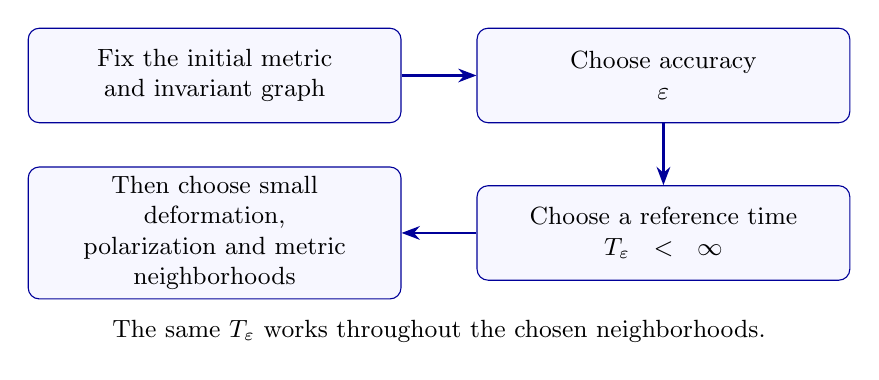
\begin{tikzpicture}[>=Stealth,
 box/.style={draw=blue!60!black,rounded corners,fill=blue!3,
  align=center,text width=4.5cm,minimum height=1.2cm,font=\small},
 arr/.style={->,thick,blue!60!black}]
\node[box] (base) at (0,0) {Fix the initial metric\\and invariant graph};
\node[box] (accuracy) at (5.7,0) {Choose accuracy\\$\varepsilon$};
\node[box] (time) at (5.7,-2) {Choose a reference time\\$T_\varepsilon<\infty$};
\node[box] (domain) at (0,-2) {Then choose small deformation,\\polarization and metric\\neighborhoods};
\draw[arr] (base.east)--(accuracy.west);
\draw[arr] (accuracy.south)--(time.north);
\draw[arr] (time.west)--(domain.east);
\node[align=center,font=\small] at (2.85,-3.25)
 {The same $T_\varepsilon$ works throughout the chosen neighborhoods.};
\end{tikzpicture}
\end{adjustbox}
\caption{The order of choices in Theorem~\ref{thm:prescribed-phase}.
The restart may depend on the prescribed metric and accuracy.
It is chosen before the small parameters, not uniformly over all
initial metrics.}
\label{fig:restart-order}
\end{figure}


\subsection{Common restart and phase for the full stable family}
\begin{theorem}\label{thm:prescribed-phase}
Fix $H^0$ as above and the graph of Theorem~\ref{thm:invariant-graph}.
There are $A,C,c,\gamma,\varepsilon_0>0$ such that for each
$0<\varepsilon<\varepsilon_0$ one can choose
$T_\varepsilon,l_\varepsilon,\rho_\varepsilon>0$ and an open
neighborhood $\mathcal U_\varepsilon$ of $W^0$ in $h^{19/8}$
with the following conclusions. For every
\begin{equation}\label{eq:prescribed-domain}
 0<l<l_\varepsilon,\qquad
 \bar x\in\mathcal B_l^{\rm st}(\rho_\varepsilon),\qquad
 W^{\rm in}\in\mathcal U_\varepsilon ,
\end{equation}
the flow from $h_0e^{W^{\rm in}}$ has a common restart
$T=T_\varepsilon$ and a selected graph trajectory $H_*(s)$,
$s\ge0$, on the same bundle, such that
\begin{equation}\label{eq:prescribed-tracking}
 \begin{gathered}
 H(T)=e^{Y_T\,*}(h_0e^{u_T}),\qquad |Y_T|_{\max}<A,\\
 v_T=u_T-\Psi(l,e^{Y_T}\bar x),\qquad
 \|v_T\|_{\mathcal E_1}<\varepsilon,\quad
 D_T=\|v_T\|_{\mathcal E_\alpha}\le\varepsilon,\\
 e^{-\eta(s)}H_*(s)\le H(T+s)\le e^{\eta(s)}H_*(s),
       \qquad\eta(s)=CD_Te^{-4cs},\\
 |Y_{\rm ph}-Y_T|\le C(|\bar x|+D_T)D_T .
 \end{gathered}
\end{equation}
The relative logarithm in the explicit frame
\eqref{eq:relative-matrix}, with actual time $T+s$, has
$h^{17/8}$ norm at most $\eta(s)$. The uniqueness class is that
of Theorem~\ref{thm:local-phase}.

For the actual and selected trace-free Dolbeault eigenvalues,
\begin{equation}\label{eq:prescribed-spectrum}
 \begin{aligned}
 \left|\log\frac{\lambda_j(T+s)}{\lambda_j^*(s)}\right|
       &\le4CD_Te^{-4cs}\quad(j\ge1),\\
 \left|\log\frac{\lambda_j(T+s)}
             {\nu_j(l,e^{Y_*(s)}\bar x)}\right|
       &\le C|\bar x|^2+CD_Te^{-4cs}\quad(1\le j\le3),\\
 \lambda_4(T+s)&\ge\gamma .
 \end{aligned}
\end{equation}
At fixed $(l,\bar x)$, the restart phase is $C^1$ in
$W^{\rm in}$ with derivative bounded uniformly over
\eqref{eq:prescribed-domain}. After a further shrinkage of
$\rho_\varepsilon$, the finite trajectory extends back to
original time zero within the reconstruction domain, and its
value there has the same $C^1$ initial-data dependence.
\end{theorem}

The fixed constants may depend on $H^0$ and the chosen graph.
The restart, neighborhoods and derivative bound may also depend
on $\varepsilon$. None requires a positive lower bound on
$\nu_1(l,\bar x)/\nu_3(l,\bar x)$. The comparison is asserted
from $T_\varepsilon$ onward, including when the finite trajectory
has been continued to an earlier time.

\begin{proof}
Choose the bound $A$ from Proposition~\ref{prop:common-entry},
then fix the local phase constants for this $A$.
Take $\varepsilon_0<\delta_A/2$. For a given $\varepsilon$,
apply the entry proposition with tolerance $\varepsilon/2$.
It selects $T_\varepsilon$ before the neighborhoods.
Retaining that time, shrink the coefficient neighborhood so
\[
 \|\Psi(l,e^{Y_T}\bar x)\|_{\mathcal E_1}
       \le Ce^{4A}|\bar x|^2<\varepsilon/2,
\]
and so that $2\rho_\varepsilon$ lies within the local phase
radius and the larger bounded diagonal translates lie within
the graph domain. This proves the first two lines of
\eqref{eq:prescribed-tracking}.
The stable balanced domain is nonempty arbitrarily near zero:
the stationary three-step family of \cite{WuebbenThreeStep26}
provides connected balanced representatives of size $O(\sqrt l)$.
The stationary equation itself forces $l\le C|\bar x|^2$,
without constraining individual positive spectral ratios.

Apply Theorem~\ref{thm:local-phase} with radius $2|\bar x|$.
Its exact reconstruction and uniqueness identify the actual
flow after restart, giving all the metric and spectral assertions.
The strong relative matrix is exactly
\eqref{eq:relative-matrix} with this shifted time origin.
The fixed-time restart map is $C^1$ by
\eqref{eq:strong-time-map} and normalization; its composition
with the local phase map gives the stated dependence.
No limiting reference diagonal has been differentiated in the
initial metric.

On $|Y|_{\max}\le A+2$ the exact finite field obeys
$\|f_{l,\bar x}\|_{C^1}\le C_{A+2}|\bar x|^2$.
The selected restart phase lies in $|Y_{\rm ph}|_{\max}<A+1/2$.
Shrink $\rho_\varepsilon$ so that
$C_{A+2}\rho_\varepsilon^2T_\varepsilon<1/4$.
A first-exit argument then continues the finite ODE backward
for time $T_\varepsilon$, within $|Y|_{\max}<A+1$.
This is backward continuation of a finite ODE, not a backward
parabolic initial-value problem. Its derivative is bounded by
$\exp(C_{A+2}\rho_\varepsilon^2T_\varepsilon)$.
Composing with the restart phase proves the original-time
assertion, without extending the small-error comparison before
entry.
\end{proof}

% Source: sections/07_spectra.tex
\section{Nonstationary spectra and equilibrium rates}\label{sec:spectra}

The spectral comparison used in the phase theorem does not require
the moving metric to be HE. The identification of finite decay rates,
by contrast, is an equilibrium assertion. We prove the two statements
separately.

\subsection{A relative estimate along the whole trajectory}
Let $D_x=d+[a(x),\,\cdot\,]$ on complex $\End_0E_0$ zero-forms.
Extend $P_0,Q_0$ complex linearly. The norms in this subsection are
the normalized spatial norms for $\omega_l$ and $h_0$.

\begin{lemma}\label{lem:full-spectrum}
There are uniform $C,\gamma,r_0>0$ such that, whenever
$|l|<l_0$, $|x|<r_0$ and $\kappa(x)=0$,
\begin{equation}\label{eq:nonstationary-spectrum}
 (1-C|x|^2)\nu_j(l,x)\le
 \lambda_j(D_x^*D_x)\le(1+C|x|^2)\nu_j(l,x)
       \quad(1\le j\le3),\qquad \lambda_4\ge\gamma .
\end{equation}
Zeros are included, and the kernel is exactly $\ker C_x$,
represented by constant diagonals. The same assertions hold with
relative error $O(|x|^2)$ for the metric $h_0e^{\Psi(l,x)}$.
More generally a change of metric with logarithmic order distance
at most $\epsilon$ changes each positive eigenvalue by a factor
between $e^{-4\epsilon}$ and $e^{4\epsilon}$.
\end{lemma}
\begin{proof}
The split Poincar\'e inequality on $Q_0$ and the smallness of $a$
give, by absorption,
\[
 \|\eta\|_{W^{1,2}}\le C\|D_x\eta\|,\qquad \eta\in Q_0W^{1,2}.
\]
For $\xi\in\mathfrak t$, equivariance gives $D_x\xi=-J_xC_x\xi$.
The harmonic orthogonality in \eqref{eq:harmonic-orthogonality}
implies
\[
 \|J_xv\|^2=(1+O(|x|^2))\|\iota v\|^2,\qquad
 |\langle J_xv,D_x\eta\rangle|
       \le C|x|\|v\|\,\|D_x\eta\|.
\]
For the second estimate, the harmonic term pairs trivially with
$d\eta$. Its pairing with $[a,\eta]$ is bounded by
$C|x|\|v\|\|\eta\|_{L^2}$. The correction $B_xv$ is $O(|x|)\|v\|$
in a fixed smooth norm and pairs with $d\eta$ by the same bound.
All constants are uniform in $l$, since the weighted harmonic
orthogonality is exact.

Minimize $\|D_x(\xi+\eta)\|^2$ over complementary $\eta$.
Complementary coercivity gives a unique linear minimizer $\eta_x\xi$,
and the variational equation and preceding pairing show
\[
 \|\eta_x\xi\|_{W^{1,2}}\le C|x|\|C_x\xi\|
                \le C|x|^2|\xi|.
\]
The minimized form $s_x$ consequently satisfies
\[
 (1-C|x|^2)\|C_x\xi\|^2\le s_x(\xi)
                  \le(1+C|x|^2)\|C_x\xi\|^2.
\]
If $C_x\xi=0$, the minimizer is zero. Conversely a zero of the
minimized form has $C_x\xi=0$, and complementary coercivity then
forces $\eta=0$. Thus the kernel assertion is exact.

On the form domain use
$T_x(\xi+\eta)=\xi+\eta_x\xi+\eta$.
It preserves that domain, differs from the identity by $O(|x|^2)$
in $L^2$, and makes the derivative-energy form the orthogonal sum
of $s_x$ and $\|D_x\eta\|^2$. The mass form changes by
$1+O(|x|^2)$. Min--max, first on this three-dimensional finite
space and then on its uniformly coercive complement, proves
\eqref{eq:nonstationary-spectrum}. This argument never divides
by a positive eigenvalue of $C_x^*C_x$.

If $e^{-\epsilon}H_1\le H_2\le e^\epsilon H_1$, the induced
endomorphism norms, on both zero-forms and one-forms, compare by
$e^{\pm2\epsilon}$. The holomorphic differential is unchanged.
Its Rayleigh quotients and then its ordered positive eigenvalues
compare by $e^{\pm4\epsilon}$. The holomorphic kernel is unchanged
as well. Apply this with
$\|\Psi(l,x)\|_{C^0}\le C|x|^2$ for the graph metric.
\end{proof}

This proof also explains why an additive estimate for the three
eigenvalues would be insufficient: its error could exceed the
smallest mode when the three scales separate.

\subsection{Exact rates at a balanced point}
Let $\bar x\in\mathcal B_l^{\rm st}(r)$ and
$\bar u=\Psi(l,\bar x)=w(l,\bar x)$.
The metric $\bar H=h_0e^{\bar u}$ is HE and
$f_{l,\bar x}(0)=0$. Write
\[
 L_{\rm dec}=-D_Yf_{l,\bar x}(0).
\]
Its eigenvalues describe linear decay of the exact finite equation.

\begin{proposition}\label{prop:equilibrium-rates}
The operator $L_{\rm dec}$ is self-adjoint for a positive inner
product on $\mathfrak t_{\RR}$ and has three positive eigenvalues
$d_1\le d_2\le d_3$ satisfying
\begin{equation}\label{eq:exact-rates}
 d_j=2\lambda_j(\bar H)
       =2\nu_j(l,\bar x)(1+O(|\bar x|^2)),\qquad 1\le j\le3 .
\end{equation}
The first equality is exact. The constants in the second are
uniform without a lower bound on any ratio of the $\nu_j$.
\end{proposition}
\begin{proof}
Differentiate the graph metric
$e^{Y\,*}(h_0e^{\Psi(l,e^Y\bar x)})$ at $Y=0$.
In the $\bar H$-isometric frame its tangent map is
\begin{equation}\label{eq:equilibrium-tangent}
 W\xi=2C_{\bar u}\xi+
          S_{\bar u}D_x\Psi(l,\bar x)C_{\bar x}\xi
       =2\xi+O(|\bar x|^2)|\xi|.
\end{equation}
The error estimate holds in $h^{19/8}$, so $W$ is injective.
Differentiating exact reconstruction at this stationary solution
gives
\[
 W D_Yf_{l,\bar x}(0)=-2\widetilde\Delta_{\bar\partial,\bar H}W.
\]
Here the tilde denotes the isometric expression in the fixed
Hermitian bundle. At an HE metric the curvature commutator vanishes;
the real metric linearization is exactly $-2\Delta_{\bar\partial}$,
which preserves Hermitian endomorphisms.

By \eqref{eq:field-expansion}, the finite derivative is
$O(|\bar x|^2)$: balance gives $|b(l)|\le C|\bar x|^2$.
The image of $W$ is therefore a three-dimensional invariant
subspace with eigenvalues of this size. Lemma~\ref{lem:full-spectrum}
gives exactly three small complex eigenvalues and a fixed fourth
gap. Adjoint conjugation commutes with this HE Laplacian, so its
small complex spectral subspace is the complexification of its
three-dimensional Hermitian part. The image of $W$ is that part.
Pull back its $L^2$ inner product by $W$. The displayed
intertwining identity proves self-adjointness and the exact
eigenvalue assertion. The relative comparison follows from
Lemma~\ref{lem:full-spectrum}.
\end{proof}

Thus $d_1^{-1}$ is the weakest linearized relaxation time.
Uniform exponential attraction to the finite graph in
Theorem~\ref{thm:local-phase} coexists with an arbitrarily large
$d_1^{-1}$. A linearized equilibrium rate alone does not specify
the time at which a nonlinear trajectory reaches a prescribed
tolerance.

\subsection{A larger initial class with constant error}
For comparison, one can dispense with proximity to the graph
if a small constant error is sufficient. Suppose
$|Y_0|_{\max}<A$, $\|u_0\|_{\mathcal E_1}<\delta$ and
$\bar x\in\mathcal B_l^{\rm st}(r)$. Start the finite graph flow
at exactly $Y_0$, without selecting its phase. At time zero its
metric and the prescribed metric have order distance at most
$\eta=C(\delta+e^{4A}r^2)$. Comparison with the equilibrium metric
confines this graph flow just as in the proof of
Theorem~\ref{thm:local-phase}; hence it exists for all future time.
Order preservation between the two exact flows gives
\[
 e^{-\eta}H_{\rm red}(t)\le H(t)\le e^\eta H_{\rm red}(t),
 \qquad
 \left|\log\frac{\lambda_j(H(t))}
                       {\nu_j(l,e^{Y_{\rm red}(t)}\bar x)}\right|
 \le4\eta+C_Ar^2,\quad 1\le j\le3.
\]
The fourth eigenvalue stays above a fixed positive constant.
This comparison does not identify a phase: a fixed nonzero error
can hide the slow tail produced by an incorrect finite initial value.
The selection argument of Section~\ref{sec:abstract-phase} is what
replaces this constant by an exponentially decreasing discrepancy
between exact reconstructed metrics.

% Source: sections/08_diamond.tex
\section{Two independent slope parameters}\label{sec:diamond}

The complete-family phase theorem follows the path $k=3l/5$.
There is also a three-layer family on which both slope parameters
vary independently. Its total arrow energy supplies a confinement
argument that is unavailable on the complete 83-dimensional space.
We retain this application separately.

\subsection{The exact three-layer presentation}
Use the same four line bundles and put $p=(k,l)$, $\sigma=k+l$,
\begin{equation}\label{eq:diamond-polarization}
 h_1=\left(1+\frac{k+5l}{24\pi}\right)^{-1},\qquad
 h_2=\left(1+\frac{5k+l}{24\pi}\right)^{-1},\qquad h_3=1 .
\end{equation}
The local construction again uses an open signed neighborhood
of zero. Its stable application has $k,l>0$. Let
$V_\diamond=V_{12}\oplus V_{13}\oplus V_{24}\oplus V_{34}$,
of complex dimensions $8,8,4,4$, and write its entries as
$z=(A,C,B,D)$. In harmonic polynomial bases write
$A=(a_0,a_1)$ and $C=(c_0,c_1)$ as pairs of cubic polynomials,
and $B=(b_0,b_1)$ and $D=(d_0,d_1)$ as pairs of linear polynomials
in the coordinates $[s:t]$ of the third $\PP^1$.
The obstruction is
\begin{equation}\label{eq:diamond-obstruction}
 \Omega(z)=a_0b_0+a_1b_1-c_0d_0-c_1d_1\in H^0(\PP^1,\cO(4)).
\end{equation}
For the current product metric define
\[
 \Gamma_p(z)=-d_{14,p}^*G_{2,p}(A\wedge B+C\wedge D).
\]
Let $N_p(z)$ have these four adjacent entries and central entry
$\Gamma_p(z)$ in block $14$. The Hodge decomposition gives
$d\Gamma_p=-(A\wedge B+C\wedge D)$ exactly when $\Omega(z)=0$.
There are no longer composable paths, so $d+N_p(z)$ is then
integrable with no further correction.

The harmonic representatives and their cohomological projections
are fixed as $p$ varies. The difference $\Gamma_p-\Gamma_0$
is closed, and $H^1(F_1F_4^{-1})=0$ makes it exact. The unique
coexact zero-form primitive $f_p$ gives the determinant-one map
\begin{equation}\label{eq:diamond-hodge-map}
 df_p(z)=\Gamma_p(z)-\Gamma_0(z),\qquad
 \Phi_p(z)=I-f_p(z)E_{14},\qquad
 (d+N_p(z))\Phi_p(z)=\Phi_p(z)(d+N_0(z)).
\end{equation}
Here $f_p$ denotes a section of the indicated line bundle;
$E_{14}$ records its block. It is quadratic in $z$, smooth in $p$,
and equivariant under constant diagonal gauges. This is an exact
map, since its square and all adjacent products with it vanish.
Write $E_{z^*}$ for the fixed reference bundle $d+N_0(z^*)$.

The central primitive is essential. For example choose equal
normalized harmonic bases on the first two factors and
\begin{equation}\label{eq:fixed-diamond}
 A=C=(s^3,0),\qquad B=D=(s,0).
\end{equation}
Both path cohomology products equal the nonzero quartic $s^4$
and cancel with the sign in \eqref{eq:diamond-obstruction}.
Their differential-form sum need not vanish. In the usual
representatives, if $\theta_i$ is the harmonic representative of
$\cO(-2)$, $\eta_i$ one of $\cO(-3)$, and $\tau_i$ the dual
$\cO(1)$ section, that sum has the factor
$(\tau_1\eta_1\wedge\theta_2-\theta_1\wedge\tau_2\eta_2)$.
The form $\tau_i\eta_i$ has harmonic projection $\theta_i$ but
is not equal to it. Evaluating at a zero of $\tau_1$ and a point
where the second term is nonzero proves nonvanishing. Thus
$\Gamma_p$ is nonzero, as in \cite[Section 6.4]{WuebbenThreeStep26}.

\subsection{Graph construction and confinement}
Apply the sliced construction of Section~\ref{sec:reduction}
with $a(x)$ replaced by $N_p(z)$ and both parameters adjoined
with zero evolution. Its hypotheses remain valid on the ambient
24-dimensional coefficient ball: the adjacent entries are
current-harmonic, the central entry is quadratic and co-closed,
the principal second jet is still removed by $S_u^{-1}$, and
the fixed differential domain and split normal gap are unchanged.
The same parameterwise tangency equation gives a chosen
$C^m$ graph $\Psi_\diamond(p,z)\in Q_0h^{19/8}$ with
$\Psi_\diamond=O(q)$, where
\[
 w=(\|A\|_p^2,\|C\|_p^2,\|B\|_p^2,\|D\|_p^2),\qquad
 q=\sum_e w_e .
\]
It is chosen before any initial metric. Its exact field
$\beta_\diamond$ is the expression in
\eqref{eq:finite-field} with this curvature and graph. In
particular
\begin{equation}\label{eq:diamond-field}
 \dot z_{ij}=(\beta_i-\beta_j)z_{ij},\qquad
 \beta_\diamond=b-Dw+E_p(z),\qquad |E_p(z)|\le Kq^2,
\end{equation}
where $D$ has columns $e_1-e_2,e_1-e_3,e_2-e_4,e_3-e_4$ and
\begin{equation}\label{eq:diamond-demand}
 b=\tfrac18(5\sigma,\,3k-5l,\,-5k+3l,\,-3\sigma).
\end{equation}
The quartic estimate follows either from the orthogonality proof
of Lemma~\ref{lem:quartic-field}, now using the current homotopy,
or from the diagonal unitary sign
$\diag(-1,1,1,-1)$: it negates every adjacent entry, preserves
the central quadratic entry, and makes the projected field even.
The exact field, rather than its displayed truncation, is used
throughout.

Let $a=(1,0,0,-1)$. Each incidence column has pairing one with
$a$, so
\begin{equation}\label{eq:height-coercivity}
 a\cdot Dw=q,\qquad \tfrac12q^2\le|Dw|^2\le2q^2 .
\end{equation}
The lower bound is Cauchy--Schwarz; the upper bound follows by
the triangle inequality and $|D_e|=\sqrt2$.

\begin{lemma}\label{lem:diamond-confinement}
There is a fixed $q_*>0$ such that every full-support integrable
trajectory of \eqref{eq:diamond-field} with initial energy $q_0$
and
\begin{equation}\label{eq:diamond-initial-energy}
 0<q_0<q_*,\qquad |b|\le q_0/(8\sqrt2)
\end{equation}
exists in the graph domain for all $t\ge0$, and $0<q(t)\le q_0$.
Every initially nonzero block remains nonzero at finite time.
\end{lemma}
\begin{proof}
The exact multiplicative equation gives
\[
 \dot q=2(Dw)\cdot\beta_\diamond
 \le-q^2+2\sqrt2|b|q+2\sqrt2Kq^3.
\]
Choose $q_*$ with $2\sqrt2Kq_*\le1/2$, and small enough that
$q\le q_*$ and $\Psi_\diamond=O(q)$ lie strictly inside the graph
and cutoff domains. At $q=q_0$ the right side is at most
$-q_0^2/4$, which excludes a first upward crossing.
The finite smooth field on the resulting closed coefficient ball
has no finite continuation obstruction. Each block is multiplied
by the exponential of a finite real integral and cannot vanish.
\end{proof}

Only the upper barrier for the total energy is used. Individual
weights may increase. No positive lower bound on a cut energy is
part of the argument.

\subsection{An open initial class and all-future comparison}
For any full-support $z^*$ with $\Omega(z^*)=0$, take a positive
determinant-one diagonal $g_{\rm in}$ such that
$z_0=g_{\rm in}z^*$ satisfies the strict energy conditions above.
Allow smooth metrics
\begin{equation}\label{eq:diamond-initial-metric}
 H^{\rm in}=(g_{\rm in}\Phi_p(z^*))^*(h_0e^{u_{\rm in}}),
 \qquad P_0u_{\rm in}=0,\quad \tr u_{\rm in}=0,\quad
 \|u_{\rm in}\|_{h^{19/8}}<\delta .
\end{equation}
As the admissible diagonal varies, this is an open class of
determinant-normalized metrics in the strong topology. Indeed the
map $(Y,u)\mapsto\log(e^Ye^ue^Y)$ has derivative $2Y+u$ at zero,
whose inverse is the $P_0,Q_0$ splitting. The inverse-function
theorem and translation by the fixed bundle maps give the claim;
the strict energy inequalities persist. The class contains
infinitely many normal directions off the graph.

Integrate $\dot g g^{-1}=\beta_\diamond(p,gz^*)$ from $g_{\rm in}$
and reconstruct
\begin{equation}\label{eq:diamond-reconstruction}
 H_{\rm red}(t)=(g(t)\Phi_p(z^*))^*
          (h_0e^{\Psi_\diamond(p,g(t)z^*)}).
\end{equation}
Let $\nu_j(w)$ be the three positive eigenvalues of the
four-vertex Laplacian with energy
$\sum_e w_e|\xi_i-\xi_j|^2$ and mass $\sum_i|\xi_i|^2$ on
$\sum_i\xi_i=0$.

For $k,l>0$, the \emph{quadratic balance} is the positive diagonal
orbit representative for which $Dw=b$. It exists and is unique
on each full-support orbit, by \cite[Section 7.1]{WuebbenThreeStep26}.
We use the subscript $\mathrm{eq}$ for its finite weights and eigenvalues.

\begin{theorem}\label{thm:diamond-comparison}
For sufficiently small fixed $q_*,\delta_*>0$, every initial
metric \eqref{eq:diamond-initial-metric} with $\delta<\delta_*$
has, for all $t\ge0$,
\begin{equation}\label{eq:diamond-comparison}
 \begin{aligned}
 e^{-\eta}H_{\rm red}(t)&\le H(t)\le e^\eta H_{\rm red}(t),
       &\eta&=\delta+C_\Psi q_0,\\
 \left|\log\frac{\lambda_j(H(t))}{\nu_j(w(t))}\right|
       &\le4\eta+C_sq_0 &&(1\le j\le3),\\
 \lambda_4(H(t))&\ge\gamma .
 \end{aligned}
\end{equation}
All constants are independent of the full-support orbit,
positive $k,l$, time and positive eigenvalue ratios.
The interval $0\le t\le2/\nu_{1,\rm eq}$ is therefore covered
with these same constants, where the subscript denotes the
quadratic balance on the same orbit.
\end{theorem}
\begin{proof}
Lemma~\ref{lem:diamond-confinement} and exact reconstruction give
an all-future graph metric. Comparing $e^{u_{\rm in}}$ and
$e^{\Psi_\diamond(p,z_0)}$ separately with the identity gives
the initial sandwich with $\eta$; no operator monotonicity of
the matrix exponential is invoked. Global metric-flow existence
and order preservation propagate it.

For the current co-closed reconstruction $N_p$, the proof of
Lemma~\ref{lem:full-spectrum} applies verbatim to its derivative:
its harmonic inclusion and coexact correction are orthogonal,
and $\|DN_p-\iota\|\le C|z|$. It gives relative error $O(q)$
and a fixed complementary gap for $h_0$. Changing to the graph
metric adds $O(q)$, and its bundle pullback is an isometry.
The metric sandwich contributes $4\eta$. Since $q(t)\le q_0$,
these are \eqref{eq:diamond-comparison}. Connected support and
the exact kernel assertion make all three finite modes positive.
Shrinking $q_*,\delta_*$ makes the transferred fourth gap uniform.

The stationary theorem \cite[Corollary 7.1]{WuebbenThreeStep26}
gives $\lambda_{1,\rm eq}/\nu_{1,\rm eq}=1+O(\sigma)$.
For small $\sigma$ this ratio is at least $1/2$, so the stated
interval contains $[0,1/\lambda_{1,\rm eq}]$.
The linearized metric rate is $2\lambda_{1,\rm eq}$ by our time
normalization. This is a covered time range, not a nonlinear
equilibration-time assertion.
\end{proof}

To see that the initial class has no implicit ratio restriction,
let $z_{\rm eq}=g_{\rm eq}z^*$ be its positive quadratic balance.
The stationary diamond result gives $q_{\rm eq}=\sigma$, and
\eqref{eq:height-coercivity} gives $|b|\le\sqrt2\sigma$.
The height gauge
\[
 g_{\rm ht}=\diag(\sqrt{32},1,1,1/\sqrt{32})
\]
multiplies all adjacent coefficients by $\sqrt{32}$ and the
central primitive by $32$. Thus $g_{\rm in}=g_{\rm ht}g_{\rm eq}$
has $q_0=32\sigma$ and satisfies the energy condition strictly.
It has an open admissible neighborhood. Taking $\delta=Bq_0$
makes every error in \eqref{eq:diamond-comparison} $O(\sigma)$.
The condition number of $g_{\rm eq}$ may diverge; all bundle
pullbacks are exact isometries in the estimates.

\subsection{An explicit separation of time scales}
For \eqref{eq:fixed-diamond}, identical normalized bases give
the cycle invariant
$\rho=w_{12}w_{24}/(w_{13}w_{34})=1$.
The balancing weights and nonzero characteristic polynomial are
\begin{equation}\label{eq:diamond-cubic}
 \begin{gathered}
 w_{\rm eq}=\tfrac18(5l,5k,3k,3l),\\
 s^3-2(k+l)s^2+
       \left(\tfrac{15}{16}(k^2+l^2)+3kl\right)s
       -\tfrac{15}{16}kl(k+l).
 \end{gathered}
\end{equation}
The weights satisfy $Dw=b$ and the cycle identity. Expanding the
weighted Laplacian determinant gives the polynomial. At $k=0$
the graph has two components, with positive eigenvalues
$3l/4$ and $5l/4$. Continuity and the product of the three roots
therefore give, as $k/l\to0$,
\[
 \nu_1/k\longrightarrow1,\qquad
 \nu_2/l\longrightarrow3/4,\qquad
 \nu_3/l\longrightarrow5/4 .
\]
The all-future comparison covers order $1/k$ even when the other
two inverse scales have order $1/l$. Figure~\ref{fig:diamond-scales}
plots this exact finite calculation.

\begin{figure}[tbp]
 \centering
 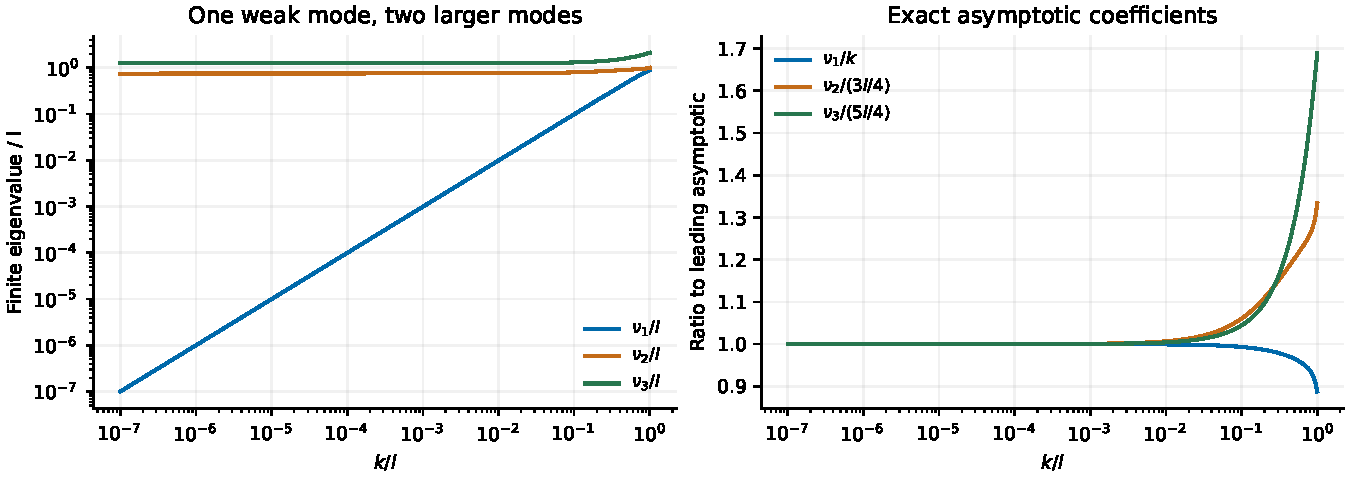
\includegraphics[width=.94\textwidth]{figures/fig03_diamond_spectra.pdf}
 \caption{The three positive finite eigenvalues for $l=1$ as
 $k/l$ decreases, and their normalized asymptotic ratios.
 Homogeneity gives every positive overall scale. The curves are
 eigenvalues of the explicit four-vertex matrix, not a numerical
 integration of HYM flow. Equation~\eqref{eq:diamond-cubic} and
 Theorem~\ref{thm:diamond-comparison} supply their analytic meaning.}
 \label{fig:diamond-scales}
\end{figure}

For a general full-support tuple, the projective direction in
each block and the positive cycle invariant $\rho$ are retained
by the exact multiplicative field. The preceding confinement and
metric comparison apply to all such tuples; the explicit polynomial
is specific to \eqref{eq:fixed-diamond}. In particular, slopes
alone do not determine a trajectory or its finite initial value.

% Source: sections/09_diamond_entry.tex
\section{Prescribed metrics on a fixed diamond bundle}\label{sec:diamond-entry}

We now hold the holomorphic bundle \eqref{eq:fixed-diamond} fixed
and remove the small-normal assumption on its initial metric.
The reference polarization is the wall $p=0$, at which this bundle
is semistable and its graded object is the locally free sum $E_0$.
The conclusion is a small constant all-future comparison after a
common restart on a full positive $(k,l)$ triangle. It is separate
from the differentiable, exponentially accurate phase theorem.

\subsection{Exact diagonal matching at the reference polarization}
Write $E=E_{z^*}$ for \eqref{eq:fixed-diamond}. Let $H_0(t)$
be its flow at $p=0$ from any smooth metric with determinant
$\det h_0$.

\begin{lemma}\label{lem:diamond-matching}
There are $T_n\to\infty$, positive constant diagonal matrices
$g_n$ with determinant one, and smooth Hermitian trace-free
fields $v_n$ such that
\begin{equation}\label{eq:diamond-matching}
 H_0(T_n)=g_n^*(h_0e^{v_n}),\qquad
 v_n\longrightarrow0\ \text{in }C^\infty,\qquad
 z_n=g_nz^*\longrightarrow0 .
\end{equation}
Each $z_n$ has full support and its central entry is exactly
$\Gamma_0(z_n)$. No bound on $g_n$, convergence rate, or
differentiable selection of this sequence is asserted.
\end{lemma}
\begin{proof}
The holomorphic flag with successive factors $F_1,F_2,F_3,F_4$
is locally free. All four slopes are zero at $p=0$, so the
bundle is semistable and this is a Jordan--H\"older filtration.
Indeed degree inequalities for a subsheaf follow by intersecting
it with the flag and adding the inequalities for its images in
the line quotients. The graded sheaf itself is $E_0$.
The corrected convergence theorem
\cite[Theorem 1.1(2) and Section 2.2]{SibleyWentworth15}
therefore has empty algebraic singular set.

The metric-to-connection isometry used in
Lemma~\ref{lem:split-metric-limit}, followed by its unitary
convergence gauges, gives complex gauges $B_n$ with
\begin{equation}\label{eq:diamond-convergence-gauge}
 B_n^*h_0=H_0(T_n),\qquad
 \mathcal D_n=B_n(d+N_0(z^*))B_n^{-1}\longrightarrow d
                 \quad\text{in }C^\infty .
\end{equation}
Here the $B_n$ need not be bounded. To obtain the much stronger
diagonal assertion, we recover the filtration and normalize its
extension representatives.

Let $i:F_1\to E$ and $p_4:E\to F_4$ be the canonical maps, and
$S_2=\ker p_4$. Cross-Hom vanishing gives
\[
 \Hom(F_1,E)=\CC i,\qquad \Hom(E,F_4)=\CC p_4,\qquad
 S_2/F_1\simeq F_2\oplus F_3 .
\]
For example $E/F_1$ has a filtration by the other three factors,
so it has no map from $F_1$. Similarly no map from $S_2$ to
$F_4$ exists. Thus the first line and last kernel are intrinsic.

Transport $i$ and $p_4$ by $B_n$ and normalize their $L^2$ norms.
After phases and a subsequence the resulting maps $i_n,p_n$
converge smoothly to the product inclusion $\iota_1$ and
projection $\pi_4$. To justify this, their zero-form Dolbeault
Laplacians have smoothly convergent coefficients by
\eqref{eq:diamond-convergence-gauge}. Elliptic estimates bound
each normalized kernel vector in every spatial norm. Each limit
has norm one in the one-dimensional split kernel, identified by
cross-Hom vanishing. This argument bounds the normalized maps,
not the gauges $B_n$.

For large $n$ the maps have constant rank. Put
\[
 j_{4,n}=p_n^*(p_np_n^*)^{-1},\qquad
 K_n=\ker p_n\cap(\im i_n)^\perp .
\]
These converge to the product fourth inclusion and middle
subbundle. Projection identifies $K_n$ smoothly with
$F_2\oplus F_3$, and its quotient Dolbeault structure tends to
the split one. The quotient is holomorphically isomorphic to
$S_2/F_1$. Normalize the generators of $\Hom(F_i,K_n)$ as
quotient maps, for $i=2,3$. The same elliptic argument makes
their lifts $j_{2,n},j_{3,n}$ converge to the middle inclusions.
They are holomorphic modulo $\im i_n$, which is sufficient.

The map $W_n=(i_n,j_{2,n},j_{3,n},j_{4,n})$ tends to the
identity. Its transported structure has split diagonal and
only entries $12,13,24,34,14$, all tending to zero. The four
adjacent entries $\alpha_{ij}$ are closed. Write
$\alpha_{ij}=\zeta_{ij}+df_{ij}$ by the reference Hodge
decomposition, with $\zeta_{ij}$ harmonic and all $f_{ij}\to0$
smoothly. Put $f=\sum f_{ij}E_{ij}$ and $U_n=I-f$.
Its inverse is exactly $I+f+f^2$ because $f^3=0$.
The transformed adjacent entries are $\zeta_{ij}$, with no
new block $23$; all new products are central. If $\chi$ denotes
the central entry after this transformation, integrability gives
\[
 d\chi=-(\zeta_{12}\wedge\zeta_{24}
                   +\zeta_{13}\wedge\zeta_{34}).
\]
Hence $\Omega(\zeta)=0$ and $\chi-\Gamma_0(\zeta)$ is closed.
Since $H^1(F_1F_4^{-1})=0$, it equals $df_{14}$ with
$f_{14}\to0$ smoothly. The further change $V_n=I-f_{14}E_{14}$
removes it. Thus $S_n=W_nU_nV_n\to I$ and
\begin{equation}\label{eq:diamond-harmonic-normalization}
 S_n^{-1}\mathcal D_nS_n=d+N_0(\zeta_n),\qquad \zeta_n\to0 .
\end{equation}

It remains to identify the resulting isomorphism
$C_n=S_n^{-1}B_n$ from the original fixed bundle.
Any such isomorphism preserves the intrinsic first line, last
kernel and the two distinct middle quotient factors. Its matrix
therefore has diagonal constants $c_i\ne0$, and only the four
adjacent and central off-diagonal entries. The adjacent
holomorphic-map equations have harmonic part
$\zeta_{ij}=(c_i/c_j)z^*_{ij}$. Their remaining part says that
the off-diagonal $C_{ij}$ are holomorphic sections, so they vanish
by cross-Hom vanishing. Diagonal covariance of $\Gamma_0$ then
makes the central map equation $dC_{14}=0$, which vanishes as
well. Thus $C_n=c_n$ is exactly constant diagonal and
$\zeta_n=c_nz^*$.

Write $c_n=J_nd_n$ with $J_n$ unitary diagonal and $d_n$ positive,
put $a_n=(\det d_n)^{1/4}$ and $g_n=a_n^{-1}d_n$.
Then
\[
 H_0(T_n)=g_n^*\widetilde h_n,\qquad
 \widetilde h_n=a_n^2J_n^*S_n^*h_0 .
\]
The determinant identity in \eqref{eq:diamond-convergence-gauge}
has $|\det B_n|=1$ pointwise. Since $S_n\to I$, it implies
$a_n\to1$. Compactness of the unitary diagonals gives
$\widetilde h_n\to h_0$ smoothly without choosing a limit of
$J_n$. Its determinant is exactly $\det h_0$. Take
$v_n=\log(h_0^{-1}\widetilde h_n)$, which is trace-free.
Finally $z_n=g_nz^*=J_n^{-1}\zeta_n\to0$; its central entry
is exactly the quadratic primitive by covariance.
\end{proof}

The three-layer recovery and the removal of the central exact
entry are essential additions to the two-step matching argument
of \cite[Lemma 8.1]{WuebbenFlow26}. Smooth connection convergence
alone would not identify these metric coordinates.

\subsection{Changing polarization at a fixed finite time}
Let $H_p^{\rm in}$ be any smooth family of determinant-normalized
metrics on this fixed bundle, extending to $p=0$, and let $H_p(t)$
be its flow. Fix a finite $T$ first. Relative to the $p$-flow,
the reference solution has metric residual
\begin{equation}\label{eq:parameter-residual}
 \begin{split}
 \mathcal R_p(t)
 &=H_0^{-1}\dot H_0+
           2(i\Lambda_pF_{H_0}-\kappa_E(p)I)\\
 &=2\{i(\Lambda_p-\Lambda_0)F_{H_0}
                  -(\kappa_E(p)-\kappa_E(0))I\}.
 \end{split}
\end{equation}
Its operator norm relative to $H_0(t)$ on $[0,T]$ is at most
$r_T(p)\le C_T|p|$. Put
$\alpha(p)=d_\infty(H_p^{\rm in},H_0^{\rm in})\to0$.
Multiplication of a metric by a spatially constant scalar leaves
its curvature unchanged, so
$e^{\pm(\alpha(p)+tr_T(p))}H_0(t)$ are respectively upper
and lower barriers for the $p$-equation. The tensor maximum
principle in \cite[Proposition 4.3 and equation (4.9)]{HKKP18}
therefore gives
\begin{equation}\label{eq:finite-time-order}
 d_\infty(H_p(t),H_0(t))\le\alpha(p)+tr_T(p),
                    \qquad 0\le t\le T .
\end{equation}
This uses the metric residual directly with its factor two,
not a conversion from a gauge-velocity error. The constant may
depend on the already chosen $T$; no infinite-time parameter
continuity is claimed.

\subsection{Restart first, then the full positive triangle}
\begin{theorem}\label{thm:diamond-prescribed}
Fix the graph $\Psi_\diamond$ and any smooth initial-metric
family $H_p^{\rm in}$ just described. For every $\epsilon>0$
there are a finite time $T_\epsilon$, a positive determinant-one
diagonal $g_\epsilon$, and $\sigma_\epsilon>0$ such that,
for every $k,l>0$ with $k+l<\sigma_\epsilon$, the exact finite
trajectory started at $g_\epsilon z^*$ at time $T_\epsilon$
has reconstruction $H_p^\epsilon(t)$ satisfying, for all
$t\ge T_\epsilon$,
\begin{equation}\label{eq:diamond-prescribed}
 \begin{aligned}
 e^{-\epsilon}H_p^\epsilon(t)&\le H_p(t)
                                  \le e^\epsilon H_p^\epsilon(t),\\
 \left|\log\frac{\lambda_j(H_p(t))}
                      {\nu_j(w_p^\epsilon(t))}\right|
      &\le\epsilon,\qquad 1\le j\le3 .
 \end{aligned}
\end{equation}
There are also fixed $T_*,\sigma_*,\gamma>0$ for this family
such that $\lambda_4(H_p(t))\ge\gamma$ for $t\ge T_*$
throughout $k,l>0$, $k+l<\sigma_*$. Neither conclusion imposes
a restriction on $k/l$.
\end{theorem}
\begin{proof}
Choose the sequence in Lemma~\ref{lem:diamond-matching} for
$H_0^{\rm in}$ and put
$q_n=\sum_e\|(g_nz^*)_e\|_0^2>0$,
$\eta_n=\|v_n\|_{\op,\infty}$.
Both tend to zero. Choose any $\delta_n\downarrow0$.
For fixed $n$ the Hodge conversion has error
\[
 c_n(p)=d_\infty((g_n\Phi_p(z^*))^*h_0,g_n^*h_0)\longrightarrow0 .
\]
This is a fixed-$n$ continuity statement and needs no uniform
bound on $g_n$. By \eqref{eq:finite-time-order} at $T_n$ and
the matching lemma, the order distance from $H_p(T_n)$ to
$(g_n\Phi_p(z^*))^*h_0$ is at most
$\eta_n+\theta_n(p)$, where
\[
 \theta_n(p)=\alpha(p)+T_nr_{T_n}(p)+c_n(p)\longrightarrow0.
\]

For all sufficiently large $n$, $q_n<q_*/4$. Shrink a full
positive triangle $k+l<\sigma_n$ until
\[
 \tfrac12q_n\le q_{n,p}\le2q_n,\qquad
 |b(p)|\le q_n/(32\sqrt2),\qquad
 \theta_n(p)\le\delta_n ,
 \qquad q_{n,p}=q_p(g_nz^*).
\]
Each condition follows from continuity at zero and $b(0)=0$.
None singles out a direction of approach. These conditions give
strictly the energy hypotheses of
Lemma~\ref{lem:diamond-confinement}.

Start the graph trajectory with $g_n$ at $T_n$.
Its energy is at most $2q_n$ for all future time. Comparing
its initial graph metric with $h_0$, then using the preceding
order bound, gives the all-future sandwich with exponent
\[
 B_n=\eta_n+\delta_n+2C_\Psi q_n\longrightarrow0 .
\]
The proof of Theorem~\ref{thm:diamond-comparison} transfers
the spectrum with error
$E_n=4B_n+2C_sq_n\to0$ and fourth gap
$e^{-4B_n}\gamma_1$. Select one index $n_*$ with $B_{n_*}<1$.
It supplies $T_*=T_{n_*}$, $\sigma_*=\sigma_{n_*}$ and
$\gamma=e^{-4}\gamma_1$. For the requested $\epsilon$, choose
$n\ge n_*$ with $E_n\le\min(\epsilon,1)$ and $B_n\le\epsilon$.
Set $T_\epsilon=T_n$, $g_\epsilon=g_n$ and
$\sigma_\epsilon=\min(\sigma_n,\sigma_*)$. All comparisons
then hold on the claimed common triangle.
\end{proof}

The theorem allows metrics outside the initial class of
Section~\ref{sec:diamond}. To see this, take a smooth real $f$
whose range contains $-1$ and $1$, and put
\[
 H^{\rm in}=h_0\exp(Mf\,\diag(1,-1,0,0)),
\]
independently of $p$.
The first column of $\Phi_p$ is the identity column. For any
metric \eqref{eq:diamond-initial-metric} with
$\|u_{\rm in}\|_{\op,\infty}<\delta_*$, the oscillation of the
logarithm of its first diagonal entry, after subtracting the
fixed reference entry, is at most $2\delta_*$. In the example
it is $2M$. Taking $M>\delta_*$ excludes that entire initial
class while preserving the theorem's hypotheses.

The restart depends on the prescribed metric and requested
accuracy. It is selected before the parameter neighborhood.
The theorem supplies no effective value of $T_\epsilon$, no
$O(\sigma)$ error at one fixed restart, and no differentiable
phase or decaying discrepancy for this two-parameter matching
sequence. Those stronger conclusions belong to
Theorem~\ref{thm:prescribed-phase} on its complete-family domain.

% Source: sections/10_compatibility.tex
\section{Compatibility of the two finite descriptions}\label{sec:compatibility}

On $k=3l/5$, the diamond lies in the complete deformation family.
Its current-Hodge reconstruction and the fixed-reference
reconstruction are related by an exact bundle map, but two chosen
parabolic graphs need not coincide. We identify a nonempty common
domain and compare their finite trajectories there.

\subsection{Bundle maps and initial-metric normalization}
On $V_\diamond$, the full reconstruction terminates at its
quadratic central term, so it is $N_0(z)$. Along the stated path,
\eqref{eq:diamond-hodge-map} gives
\begin{equation}\label{eq:compat-hodge-bounds}
 \|\Phi_l(z)-I\|_{h^{19/8}}\le Cl|z|^2,\qquad
 \|D_z\Phi_l(z)\|\le Cl|z|,\qquad
 \Phi_l(gz)=g\Phi_l(z)g^{-1}.
\end{equation}
These estimates follow by differentiating the smoothly
parameter-dependent Hodge primitive at $l=0$; it is quadratic
in $z$. The polynomial formula defines the map at a fixed
original $z^*$ even when that coordinate is not small.

Let $z_{\rm eq}=g_{\rm eq}z^*$ be a full-support quadratic
balance. Here $\sigma=8l/5$ and $q_l(z_{\rm eq})=\sigma$.
The stationary theorem supplies an actual HE metric
$\widehat H_{\rm eq}$ on $d+N_l(z_{\rm eq})$ whose logarithm
relative to $h_0$ is $O(\sigma)$ in $h^{19/8}$.
Pull it back by $\Phi_l(z_{\rm eq})$ and normalize by a positive
diagonal $S=e^{Y_{\rm eq}}$:
\begin{equation}\label{eq:compat-balance}
 P_0\log\!\left(S^{-1}
        (h_0^{-1}\Phi_l(z_{\rm eq})^*\widehat H_{\rm eq})
                         S^{-1}\right)=0,\qquad
 |Y_{\rm eq}|\le C\sigma .
\end{equation}
The derivative in $Y_{\rm eq}$ at the identity is $-2I$;
the small metric logarithm and the implicit-function theorem
give the uniform bound. Thus
$\bar x=Sz_{\rm eq}\in\mathcal B_l^{\rm st}$ and
$|\bar x|\le C_0\sqrt\sigma$. The fixed holomorphic map
$F=Sg_{\rm eq}$ identifies $E_{z^*}$ with $E_{\bar x}$.
This is a bundle isomorphism, with the corresponding metric
pullback; no estimate for the condition number of $g_{\rm eq}$
is used.

Take a diamond initial metric
$(g_{\rm old}\Phi_l(z^*))^*(h_0e^v)$ with $P_0v=0$.
Put $z_{\rm old}=g_{\rm old}z^*$ and
$d_{\rm in}=g_{\rm old}g_{\rm eq}^{-1}S^{-1}$.
On $E_{\bar x}$ that same metric is exactly
\begin{equation}\label{eq:compat-initial}
 d_{\rm in}^*\bigl(\Phi_l(z_{\rm old})^*(h_0e^v)\bigr).
\end{equation}
Let $e^w=\Phi_l(z_{\rm old})^*e^v\Phi_l(z_{\rm old})$ in
$h_0$ frames, and choose a real constant diagonal $Z$ with
\[
 u=\log(e^{-Z}e^we^{-Z}),\qquad P_0u=0.
\]
Because $P_0v=0$, \eqref{eq:compat-hodge-bounds} and the same
normalization derivative give
\begin{equation}\label{eq:compat-normalization}
 |Z|\le Clq_0,\qquad
 \|u\|_{h^{19/8}}\le C(\|v\|_{h^{19/8}}+lq_0),\qquad
 g_{\rm in}=e^Zd_{\rm in},\quad q_0=q_l(z_{\rm old}).
\end{equation}
Equations \eqref{eq:compat-initial}--\eqref{eq:compat-normalization}
place exactly the same initial metric in the full-family
coordinates of \eqref{eq:local-initial}.

\subsection{A common domain without a spectral-ratio bound}
Fix $A_0>\log\sqrt{32}$ and $B>0$. Impose
\begin{equation}\label{eq:common-domain}
 \begin{gathered}
 |\log(g_{\rm old}g_{\rm eq}^{-1})|_{\max}<A_0,\qquad
 q_0<q_*,\qquad |b(l)|<q_0/(8\sqrt2),\\
 \|v\|_{h^{19/8}}<B\sigma .
 \end{gathered}
\end{equation}
Then $q_0\le e^{4A_0}\sigma$. Choose
$A=A_0+1$ and $r=2C_0\sqrt\sigma$. The graph and
\eqref{eq:compat-normalization} give
$\|u-\Psi(l,g_{\rm in}\bar x)\|_{\mathcal E_1}
\le C_{A_0,B}\sigma$.
For sufficiently small $\sigma$, these are the hypotheses of
Theorem~\ref{thm:local-phase}. Every bound is independent of
the cycle invariant $\rho$ and the positive finite spectral ratios.
The height choice $g_{\rm old}=g_{\rm ht}g_{\rm eq}$ has
$q_0=32\sigma$ and lies strictly inside
\eqref{eq:common-domain}, so this is a nonempty open common domain.

Both time conventions are \eqref{eq:hym-flow}; the normalized
harmonic norms agree on the selected subspace. The full-family
phase theorem therefore gives the same $O(\sigma)$ spectral
and metric comparison on these actual bundles, with its additional
decaying comparison to the selected exact trajectory. At
equilibrium \eqref{eq:compat-balance} changes the finite form
only by relative $1+O(\sigma)$. Proposition~\ref{prop:equilibrium-rates}
then gives
\[
 d_j=2\nu_j(z_{\rm eq})(1+O(\sigma)),\qquad 1\le j\le3 ,
\]
and the same estimates cover $0\le t\le2/\nu_1(z_{\rm eq})$.

\subsection{Comparing the chosen graph trajectories}
Convert the diamond graph flow to $E_{\bar x}$ by $F$.
At each time normalize it as in
\eqref{eq:compat-normalization}, now with
$v=\Psi_\diamond(l,z_{\rm old}(t))$. Its exact metric becomes
\[
 \widetilde g(t)^*(h_0e^{\widetilde u(t)}),\qquad
 \widetilde x(t)=e^{Z(t)}z_{\rm old}(t)
                         =\widetilde g(t)\bar x .
\]
Diamond confinement gives
$q_l(z_{\rm old}(t))\le q_0$, hence
$\|\widetilde u(t)\|_{C^0}\le Cq_0$ and $|Z(t)|\le Clq_0$.
The selected full-family graph metric and this converted graph
metric are both exact flows on $E_{\bar x}$. Their initial
order distance is $O_{A_0,B}(\sigma)$, by comparison with
\eqref{eq:compat-initial}; order preservation propagates that
bound for all future time.

Both complementary metric logarithms are $O(\sigma)$.
Comparing their positive diagonal squares with $h_0$ therefore
gives
\begin{equation}\label{eq:compatible-trajectories}
 |\log g_*(t)-\log\widetilde g(t)|_{\max}
       \le C_{A_0,B}\sigma,\qquad
 x_*(t)=e^{\Theta(t)}z_{\rm old}(t),\qquad
 |\Theta(t)|_{\max}\le C_{A_0,B}\sigma .
\end{equation}
Indeed insert the separate estimates
$e^{-C\sigma}h_0\le h_0e^{\Psi},h_0e^{\widetilde u}
\le e^{C\sigma}h_0$ into the metric sandwich. The diagonal
squares commute, and their scalar logarithms differ by
$O(\sigma)$. No derivative of $Z$ divided by a weak mode,
and no inverse orbit form, occurs. Every edge energy and the
entire finite form consequently compare by $e^{\pm C\sigma}$.
Min--max gives that comparison for every positive finite eigenvalue.

The result is compatibility of exact bundle presentations,
time normalizations, actual flows and finite spectra on their
common domain. It does not identify the two independently chosen
invariant graphs. The prescribed-metric theorem of
Section~\ref{sec:diamond-entry} retains its larger independent
two-parameter domain; it is not a consequence of restriction
to the single path used by the complete-family phase theorem.

\FloatBarrier
\begin{thebibliography}{Wue26c}

\bibitem[HKKP18]{HKKP18}
F.~Haiden, L.~Katzarkov, M.~Kontsevich and P.~Pandit,
\emph{Iterated logarithms and gradient flows}, preprint, 2018,
\href{https://arxiv.org/abs/1802.04123v1}{arXiv:1802.04123v1}.

\bibitem[Kob87]{Kobayashi87}
S.~Kobayashi, \emph{Differential Geometry of Complex Vector Bundles},
Publications of the Mathematical Society of Japan, vol.~15,
Kan\^o Memorial Lectures, vol.~5, Iwanami Shoten and Princeton
University Press, 1987.
\href{https://www.mathsoc.jp/assets/pdf/publications/pubmsj/Vol15.pdf}
{Official Mathematical Society of Japan edition}.

\bibitem[Lam26]{Lam26}
S.~T.~Lam, \emph{Semistability and asymptotics of geometric flows},
preprint, 2026,
\href{https://arxiv.org/abs/2606.09235v1}{arXiv:2606.09235v1}.

\bibitem[SS14]{ShaoSimonett14}
Y.~Shao and G.~Simonett,
\emph{Continuous maximal regularity on uniformly regular
Riemannian manifolds}, J. Evol. Equ. \textbf{14} (2014), no.~1,
211--248.
\href{https://doi.org/10.1007/s00028-014-0218-6}
{doi:10.1007/s00028-014-0218-6}.
Locators refer to
\href{https://arxiv.org/abs/1309.2041v1}{arXiv:1309.2041v1}.

\bibitem[SW15]{SibleyWentworth15}
B.~Sibley and R.~A.~Wentworth,
\emph{Analytic cycles, Bott--Chern forms, and singular sets for
the Yang--Mills flow on K\"ahler manifolds},
Adv. Math. \textbf{279} (2015), 501--531.
\href{https://doi.org/10.1016/j.aim.2015.04.009}
{doi:10.1016/j.aim.2015.04.009}.
The corrected text and appended erratum are
\href{https://arxiv.org/abs/1402.3808v3}{arXiv:1402.3808v3}.

\bibitem[Sim94]{Simonett94}
G.~Simonett, \emph{Invariant manifolds and bifurcation for
quasilinear reaction-diffusion systems}, Nonlinear Anal.
\textbf{23} (1994), no.~4, 515--544.
\href{https://doi.org/10.1016/0362-546X(94)90092-2}
{doi:10.1016/0362-546X(94)90092-2}.

\bibitem[Sim95]{Simonett95}
G.~Simonett, \emph{Center manifolds for quasilinear
reaction-diffusion systems}, Differential Integral Equations
\textbf{8} (1995), no.~4, 753--796.
\href{https://doi.org/10.57262/die/1369055610}
{doi:10.57262/die/1369055610}.

\bibitem[Wue26a]{WuebbenThreeStep26}
B.~J.~Wuebben, \emph{Hermitian--Einstein metrics and small spectra
for three-step extensions}, preprint, October 31, 2026.
\href{https://doi.org/10.5281/zenodo.23850990}{doi:10.5281/zenodo.23850990}.

\bibitem[Wue26b]{WuebbenFlow26}
B.~J.~Wuebben, \emph{Metric response and Hermitian Yang--Mills
flow for two-step extensions}, preprint, October 27, 2026.
\href{https://doi.org/10.5281/zenodo.23717742}
{doi:10.5281/zenodo.23717742}.

\bibitem[Wue26c]{WuebbenWall26}
B.~J.~Wuebben, \emph{$L^2$ metrics on Hermitian--Yang--Mills moduli spaces near a stability wall},
preprint, October 31, 2026.
\href{https://doi.org/10.5281/zenodo.23850992}{doi:10.5281/zenodo.23850992}.

\end{thebibliography}

\end{document}
